\chapter{Techno-ökonomische Optimierung}\label{chapter: Techno-ökonomische Betriebsmodelle}
\thispagestyle{empty}
Abbildung \ref{fig: Schema_Optimierung} zeigt das grundsätzliche Vorgehen bei der Optimierung von Energiesystemen. In der Vorbereitung werden die benötigten Daten gesammelt und für die Optimierung entsprechend aufbereitet. Diese Parameter werden dem Modell des Energiesystems als Eingangsdaten zugeführt und innerhalb des Modells genutzt, um entsprechende Randbedingungen für die Einsatzoptimierung zu generieren. Bei der Optimierung wird nun die kostenoptimale Deckung des vorgegebenen Wärmebedarfs bestimmt. Zur Lösung des Optimierungsproblems ist der kommerzielle Solver gurobi \cite{gurobi} verwendet worden, der zu akademischen Zwecken kostenfrei genutzt werden kann. Um die Dauer der Optimierung zu verringern, ist die Genauigkeit des Solvers auf 1\% limitiert worden. Als Ergebnis der Optimierung können beispielsweise die Laufzeiten der Anlagen, der Speicherfüllstand oder der Erlös des Energiesystems ausgelesen werden.
	\begin{figure}[ht]
		\centering
		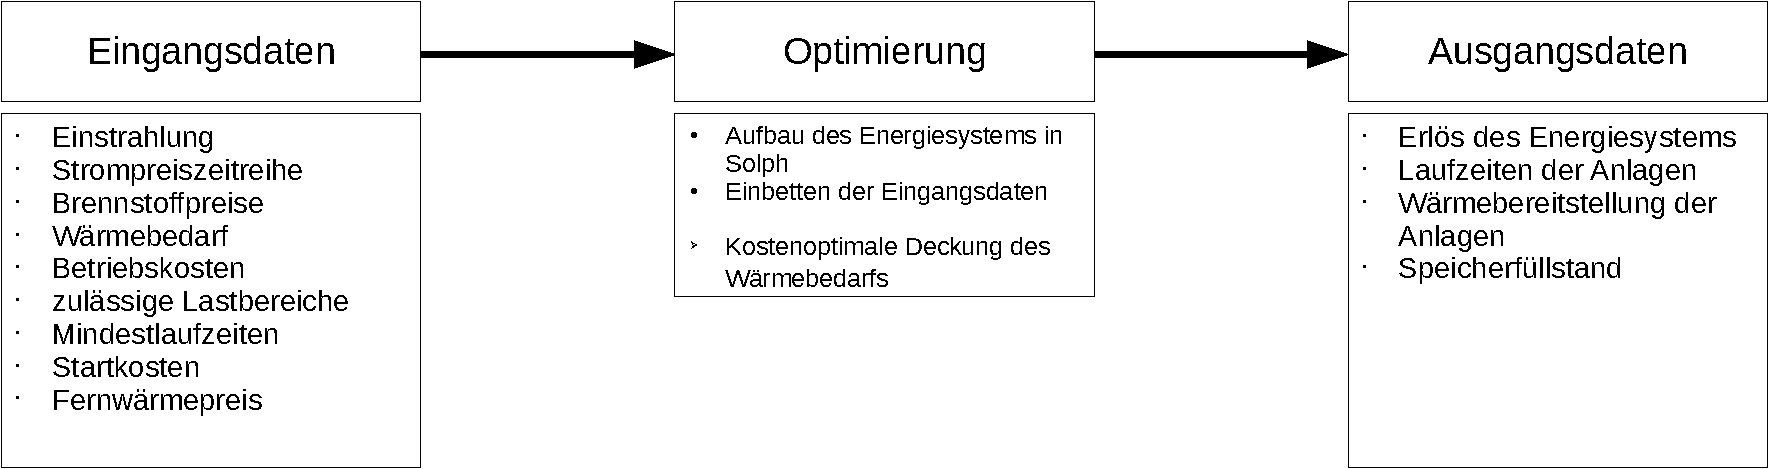
\includegraphics[width=1\linewidth]{Schema_Optimierung.pdf}
		\captionof{figure}{Grundsätzlicher struktureller Aufbau der Betriebsoptimierung}
		\label{fig: Schema_Optimierung}
	\end{figure}

In diesem Kapitel wird gezeigt wie die Konzepte der solarthermischen Wärmebereitstellung in techno-ökonomische Betriebsmodelle überführt worden sind und mit welchem Ergebnis diese Modelle optimiert wurden. Die Ergebnisse der jeweiligen Optimierung werden bewertet und vergleichend in einen größeren Kontext eingeordnet. Zu diesem Zweck wird zunächst die Software Solph vorgestellt, die genutzt worden ist, um die Energiesysteme zu erstellen und zu optimieren. 

Im Anschluss daran werden die Eingangsdaten der durchgeführten Optimierungen genauer betrachtet. In den folgenden Abschnitten wird dann zunächst das Referenzsystem vorgestellt, welches repräsentativ für konventionelle, auf fossilen Brennstoffen basierenden, Wärmeversorgungssysteme in Deutschland stehen soll, bevor die zuvor ausgewählten Alternativsysteme untersucht werden.

\section{Optimierungssoftware Solph}\label{section: Solph}
Solph ist ein Python-Paket des \acf{oemof}, welches vom \citet{RLI2019} und dem \citet{ZNES2019} entwickelt worden ist, um lineare und gemischt-ganzzahlige Probleme zu erstellen und über einen Solver zu lösen. In Solph lassen sich vordefinierte Komponenten miteinander verschalten, um ein Energiesystem aufzubauen. Im Hintergrund wird aus dem erstellten System und den Eingangsdaten die in Kapitel \ref{section: Optimierungsverfahren} beschriebene Zielfunktion und die entsprechenden Nebenbedingungen eines linearen Problems erstellt. Dieses, durch Solph automatisch generierte, lineare Modell wird nun über ein anderes Python-Paket, welches nicht Teil des \acl{oemof} ist, gelöst. Hierbei handelt es sich um Pyomo \cite{hart2017pyomo}, auf das an dieser Stelle nicht weiter eingegangen und auf die entsprechende Dokumentation verwiesen wird. 
	\begin{figure}[ht]
		\centering
		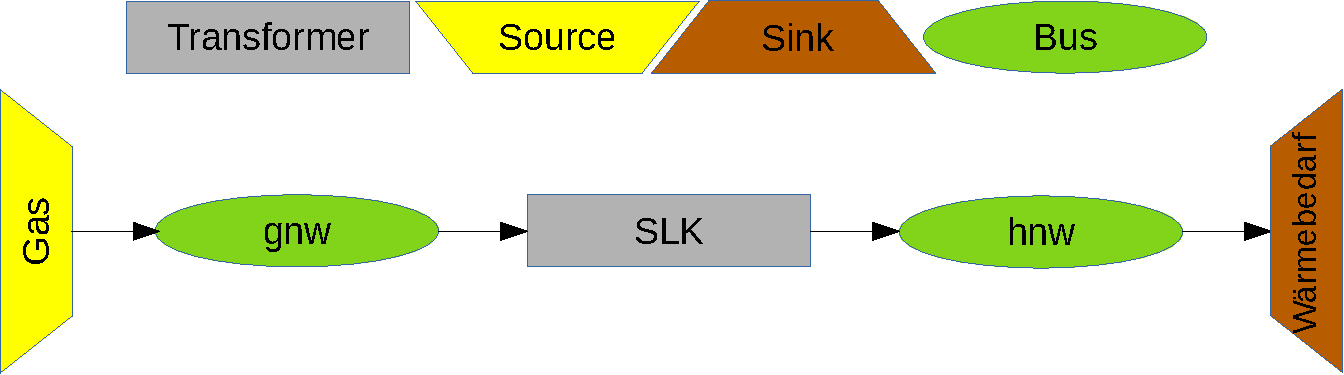
\includegraphics[width=0.8\linewidth]{Solph_Bsp.pdf}
		\captionof{figure}[Schaltlogik eines einfachen Energiesystems in Solph]{Schaltlogik eines einfachen Energiesystems in Solph. Eine Gasquelle ist als Source dargestellt und kann einen Bus, in diesem Fall das Gasnetzwerk (gnw), mit Gas beliefern. Ein Spitzenlastkessel wandelt die Energie des Gases in Wärme um und versorgt das Heiznetzwerk (hnw), aus dem schließlich der Wärmebedarf gedeckt wird.}
		\label{fig: BSP in Solph}
	\end{figure}

In Abbildung \ref{fig: BSP in Solph} wird gezeigt, wie prinzipiell einzelne Anlagen in Solph verschaltet werden können, um ein Energiesystem abzubilden. Dabei stellen Transformer Anlagen dar, die mit einem gewissen Wirkungsgrad (conversion factor) eine oder mehrere Eingangsgrößen transformieren und entsprechende Ausgangsgrößen bereitstellen. Im gezeigten Beispiel ist der \ac{SLK} ein Transformer, der Gas aus dem Gasnetzwerk (gnw) bezieht und die aus dem Gas bezogene Energie in Wärme umwandelt und dem Heiznetzwerk (hnw) zuführt. Aus dem Heiznetzwerk wird nun der Wärmebedarf gedeckt.

Die Verbindungen zwischen den einzelnen Komponenten des Energiesystems werden als Flow bezeichnet und stellen den Energiestrom zwischen verschiedenen Komponenten dar. Je nach Ziel der Optimierung ist es genauso möglich Stoffströme abzubilden, beispielsweise Abgase oder Ware einer Produktion.

Die Flows können mit Kosten oder einem Erlös pro bereitgestellter Einheit belegt werden, so ist es beispielsweise möglich den Flow zwischen der Gas-Source und dem Gasnetzwerk mit einem Gaspreis pro MWh zu belegen. Dieser Wert muss nicht konstant sein. Es können dem Modell auch Preiszeitreihen in stündlicher Auflösung übergeben werden. Dies ist beispielsweise bei dem durch den Börsenhandel volatilen Strompreis der Fall. Zusätzlich können über die Flows variable Betriebskosten der einzelnen Anlagen, maximale bzw. minimale Laufzeiten, eine minimale bzw. maximale Leistung oder Startkosten hinzugefügt werden. Dies sind Parameter aus denen Solph die entsprechenden Randbedingungen für die Optimierung erstellt.

Im folgenden wird kurz gezeigt, wie in Solph ein Energiesystem erstellt werden kann. Diese Betrachtung ist stark an die Solph-Dokumentation \cite{oemof2019} angelegt und für eine genauere Betrachtung wird an eben diese verwiesen. 

Zunächst ist ein Betrachtungszeitraum für die Optimierung erforderlich. Dieser kann über das Python-Paket Pandas erstellt werden. Hier wird, ausgehend von einem Startdatum, der Zeitraum über die Anzahl der Intervalle \textit{periods} und die Schrittweite \textit{freq} (h=Stunden) definiert. In diesem Beispiel ist der Zeitraum 24 Stunden vom 01. Januar 00:00 Uhr:
\begin{lstlisting}[language=python,numbers=none]
import pandas as pd
time_index = pd.date_range('1/1/2016 00:00:00', periods=24, freq='h')
\end{lstlisting}
Dieser Betrachtungszeitraum wird nun genutzt, um ein Energiesystem zu erstellen:
\begin{lstlisting}[language=python,numbers=none]
import oemof.solph as solph
es = solph.EnergySystem(timeindex=time_index)
\end{lstlisting}
Dieses Energiesystem ist leer und enthält nichts weiter als eine Information über den Optimierungszeitraum. In einem nächsten Schritt können dem System nun die gewünschten Komponenten -Bus, Transformer, Source und Sink- hinzugefügt werden:
	\begin{lstlisting}[language=python,numbers=none]
# Source and Sink
gas_source = solph.source(label='gas source',
				outputs={gnw: solph.Flow(variable_costs=1)})
heat_sink = solph.sink(label='heat_sink',
				inputs={hnw: solph.Flow(actual_value=Bedarf, fixed=True)})					   
es.add(gas_source, heat_sink)
		
# Busses
gnw = solph.Bus(label='gas_network')
hnw = solph.Bus(label='heat_network')
es.add(gnw, enw, hnw)
	
# Transformer
SLK = solph.Transformer(label='Spitzenlastkessel',
						inputs={gnw: solph.Flow()},
						outputs={hnw: solph.Flow(nominal_value=30,
											variable_costs=1)},
		  							  conversion_factors={hnw: 0.88})
es.add(SLK)
\end{lstlisting}
In diesem Beispiel ist dem Energiesystem nun eine Gasquelle hinzugefügt worden, aus der bei Bedarf Gas mit einem Preis von 1 pro Einheit bezogen und dem Gasnetzwerk zugeführt wird. An dieser Stelle liegt es an dem Modellierer, welche Einheit die \textit{variable costs} erhalten - es können beispielsweise €/kWh oder €/MWh sein. Die Einheit muss jedoch für das gesamte Modell einheitlich gewählt werden.

Der Spitzenlastkessel bezieht sein Gas aus dem Gasnetzwerk und stellt mit einem Wirkungsgrad von 88\% einen Wärmestrom bereit, der ans Heiznetzwerk abgegeben wird. Der Nenn-Wärmestrom beträgt in diesem Fall 30 - die Einheit ist wieder frei wählbar. Wichtig ist nur, dass die Einheit mit dem Gaspreis zusammenpasst, um plausible Ergebnisse zu erhalten.  
Der Wärmebedarf deckt sich nun aus dem Heiznetzwerk. Durch den Befehl \textit{fixed=True} wird vorgegeben, dass der Bedarf gedeckt sein muss. Das heißt, dass dieser Senke nicht mehr oder weniger Wärme zugeführt werden darf, als benötigt.

Das nun erstellte Netzwerk kann unter Verwendung eines geeigneten Solvers - in diesem Fall des Gurobi-Solvers - gelöst werden:
\begin{lstlisting}[language=python,numbers=none]
model = solph.Model(es)
model.solve(solver="gurobi")
\end{lstlisting}
Im Postprocessing können nun die Ergebnisse der Einsatzoptimierung über weitere Pakete des \acl{oemof} verarbeitet und dargestellt werden.

\section{Eingangsparameter der Optimierung}\label{section: Eingangsparameter der Optimierung}
Die Eingangsparameter der Optimierung können eigene Prognosen oder historische Parameter aus vergangenen Jahren sein. Im Rahmen dieser Arbeit ist das Jahr 2016 als Betrachtungszeitraum gewählt worden, weshalb alle Eingangsdaten aus diesem Zeitraum stammen. Dieser Abschnitt wird die verwendeten Wetterdaten, Preiszeitreihen und Wärmelast kurz vorstellen. Sollten die Daten vor oder nach der Optimierung verwendetet worden sein, wird dieser Abschnitt außerdem erläutern wie dies erfolgt ist. Alle hier aufgeführten Daten können ebenfalls dem beigelegten Datenträger entnommen werden.

Kosten beschreibende Parameter, wie beispielsweise Betriebskosten oder Energiekosten, fließen mit positivem Vorzeichen in die Optimierung ein. Dementsprechend werden alle Parameter, die Einnahmen verursachen - Fernwärmepreise und Stromvermarktung - mit negativem Vorzeichen berücksichtigt.

\subsection*{Wetterdaten}
Für den Betrieb der Solarthermieanlagen sind die standortbezogenen Umgebungsbedingungen entscheidend. Dies sind die Umgebungstemperatur und Sonneneinstrahlung. Die Umgebungstemperatur kann standortspezifisch und unentgeltlich auf der Internetseite Renewables.ninja \cite{pfenninger2016renewables} heruntergeladen werden. Die zugänglichen Daten stellt das MERRA-2 Projekt der Nasa \cite{Gelaro2017a} zur Verfügung. Registrierte Benutzer können die Temperaturen in stündlicher Auflösung für die Jahre 2000 bis 2018 erhalten. Zusätzlich zur Umgebungstemperatur können Daten zu der Bewölkung, der Einstrahlung am Boden und einigen weiteren Parametern abgerufen werden. 

Bei der Sonneneinstrahlung von Renewables.ninja wird jedoch nicht zwischen direkter und diffuser Strahlung unterschieden. Diese Daten lassen sich deshalb nur bedingt weiter verwenden, da bei der Umrechnung von horizontaler in die direkte Einstrahlung Kenntnis über den Diffus-Anteil erforderlich ist. Aus diesem Grund ist für die Einstrahlung ein Datensatz des Deutschen Wetterdienstes verwendet worden. Dieser stellt für ausgewählte Standorte in Deutschland Wetterdaten von 1980 bis 2018 bereit \cite{DWDstrahlung}. Der Standort Schleswig ist repräsentativ für norddeutsche Strahlungsverhältnisse ausgewählt worden.

Die Strahlungsdaten für die horizontale Ebene sind in einem Python-Skript auf eine geneigte Ebene nach dem in Kapitel \ref{Funktionsweise Solarthermische Wärmebereitstellung} vorgestellten DIN-Algorithmus umgerechnet worden. Das Skript ist dem Anhang \ref{Anhang: Sonnenstand} oder dem beigefügten Datenträger zu entnehmen. Die Umgebungstemperatur und Einstrahlung auf die geneigte Ebene sind im Preprocessing genutzt worden, um den Ertrag der Solarthermie zu berechnen. Der so ermittelte, stündlich aufgelöste, Wärmestrom pro m$^2$ wurde schließlich an die Optimierungsmodelle übergeben. Im Fall der Photovoltaik ist ausschließlich die Einstrahlung zur Berechnung der elektrischen Leistung, welche an das Optimierungsmodell übergeben wird, verwendet worden.

\subsection*{Heizlast, Vor- und Rücklauftemperaturen des Wärmenetzes}
Die Stadtwerke Flensburg haben für die Jahre 2014 bis 2016 Daten zu ihrem Fernwärmenetz bereitsgestellt \cite{stadtwerke_flensburg_gmbh_2019_2553968}. Diese beinhalten die Rück- und Vorlauftemperaturen, sowie die Heizlast des Netzes. Diese Daten sind in Bezug auf das Temperaturniveau und den Verlauf der Heizlast als repräsentativ für typische Wärmenetze Norddeutschlands angenommen worden. Die Heizlast ist nach der Einwohnerzahl normiert worden wobei davon ausgegangen wurde, dass die Stadtwerke Flensburg ca. 100.000 Einwohner mit Fernwärme versorgen.

Die größte solarthermische Anlage Deutschlands, mit einer Fläche von 8.300 m$^2$, steht in Senftenberg \cite{SDH2019}. Das Wärmenetz versorgt 25.000 Einwohner und erreicht dabei eine \ac{SF} von 4\% \cite{Senftenberg}. Die Heizlast, die im Rahmen dieser Arbeit zur Optimierung verwendet wird, ist auf eine Einwohnerzahl von ca. 50.000 skaliert worden. Somit wurde die Flensburger Last halbiert. Die Skalierung wurde vor dem Hintergrund gewählt, dass das im Rahmen dieser Arbeit betrachtete Netz größer als bisherige solarthermisch unterstützte Netze in Deutschland ausfallen sollte, aber nicht unrealistisch groß. Prinzipiell kann die Heizlast in Norddeutschland aber auf jede Netzgröße skaliert werden. Abbildung \ref{fig: Heizlast} stellt den Verlauf der gewählten Heizlast grafisch dar. 
	\begin{figure}[ht]
		\centering
		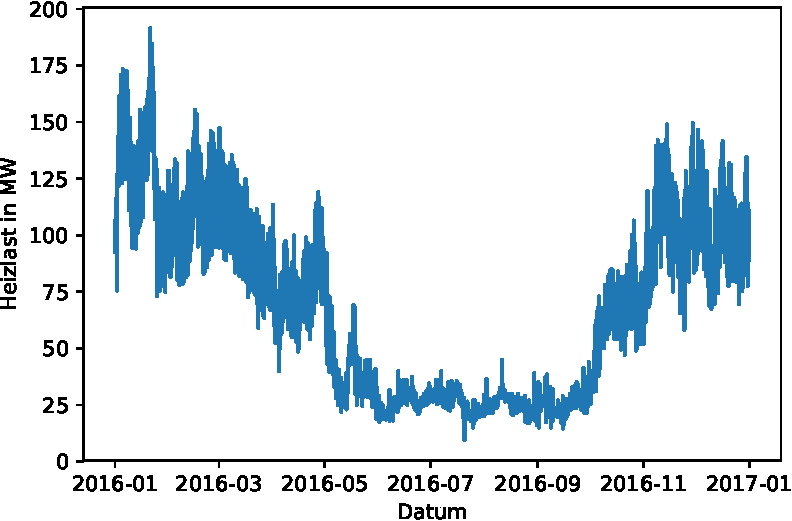
\includegraphics[width=0.8\linewidth]{HL.pdf}
		\captionof{figure}{Darstellung des Verlaufs der Heizlast des untersuchten Wärmenetzes für das Jahr 2016}
		\label{fig: Heizlast}
	\end{figure}

Die Rücklauftemperatur des Netzes wird konstant auf 50\textdegree C gehalten. Die Vorlauftemperatur erreicht im Winter 124\textdegree C und fällt im Sommer auf durchschnittlich 80\textdegree C ab. Diese Temperaturen sind unverändert aus dem Stadtwerke Flensburg Datensatz übernommen und wurden bei der Berechnung des von den Solarkollektoren abgegebenen Wärmestroms genutzt.

\subsection*{Preiszeitreihen Strom, Gas und Fernwärme}
In dieser Arbeit werden folgende Preiszeitreihen benötigt:
	\begin{description}
		\item[Fernwärmepreis] Der Fernwärmepreis ist bei der durchgeführten Optimierung als konstanter Wert angenommen worden. Aus \citet{Kaldemeyer2019} ist ein durchschnittlicher Fernwärmepreis für das Jahr 2016 von 68,59 \euro/MWh übernommen worden.
		\item[Gaspreis] Bei dem Gaspreis wird ebenfalls von einem konstanten Gaspreis über den Betrachtungszeitraum ausgegangen. Die \ac{PEGAS} veröffentlicht den nach Monaten und Jahren aufgeschlüsselten \ac{EGIX} ab dem Jahr 2008. Für die durchgeführte Einsatzoptimierung ist der Durchschnittswert für das Jahr 2016 von 14,14 \euro/MWh verwendet worden. \cite{GasPrice}
		\item[Strompreis (Verkauf)] Im Rahmen dieser Arbeit ist ausschließlich die Stromvermarktung über Day-Ahead Auktionen an der europäischen Strombörse betrachtet worden. Eine stündlich aufgelöste Preiszeitreihe über die Day-Ahead-Strompreise aus dem Jahr 2016 ist dem Agorameter \cite{Agora2016} entnommen worden.
		\item[Strompreis (Bezug)] Der aus dem elektrischen Netz bezogene Strom setzt sich aus der Strompreiszeitreihe für den Verkauf und Stromabgaben\footnote{Stromabgaben setzten sich zusammen aus: EEG-Umlage, Konzessionsabgabe, KWKG-Umlage, §19 StromNEV-Umlage, Offshore-Netzumlage, Stromsteuer} zusammen. Für die Stromabgaben ist ein konstanter Wert von 85,51 \euro/MWh angenommen worden, welcher der Strompreisanalyse des Bundesverbands der Energie- und Wasserwirtschaft \cite{BDEW} entnommen wurde. 
	\end{description} 

\subsection*{Betriebskosten, CO$_2$-Zertifikat, Energiesteuer}
Unter diesem Abschnitt werden alle Kosten, die beim Betrieb der technischen Anlagen anfallen, aufgeführt. Diese reichen von den Betriebskosten, die den Verschleiß und die notwendige Wartung der Anlage berücksichtigen, über CO$_2$-Zertifikatspreise pro t$_{\text{CO}_2}$ zu einer Energiesteuer beim Betrieb eines Spitzenlastkessels. Zunächst sollen die Betriebskosten der Anlagen und ihr Zustandekommen genauer betrachtet werden.
\subsubsection*{Solarthermie / Photovoltaik}
Nach Angaben des Fraunhofer-Instituts für solare Energiesysteme können für den Betrieb von \ac{PV}-Anlagen Kosten in Höhe von 1\% der Investitionskosten angenommen werden \cite{ISE}. Dieser Wert ist für den Betrieb der solarthermischen Anlagen übernommen worden. Die Betriebskosten BK errechnen sich dann über den Quotienten aus dem im Preprocessing ermittelten Ertrag $Q_\text{ST}$ / $W_\text{PV}$ der Anlage und den Investitionskosten $I$. Dies wird in Gleichung \ref{equation: Betriebskosten Solar} und \ref{equation: Betriebskosten PV} veranschaulicht. 
	\begin{align}
		\label{equation: Betriebskosten Solar}
		\text{BK}_\text{ST} &= \dfrac{0,01 \cdot I_\text{ST}}{Q_\text{ST}} \hspace{1cm} [\euro/\text{MWh}]\\
		\label{equation: Betriebskosten PV}
		\text{BK}_\text{PV} &= \dfrac{0,01 \cdot I_\text{PV}}{W_\text{PV}} \hspace{1cm} [\euro/\text{MWh}]
	\end{align}
Die Investitionskosten der Anlagen werden nach den in Kapitel \ref{subsection: Kostendegression} vorgestellten Gleichung ermittelt.

\subsubsection*{Wärmespeicher}
Für den \ac{STES} sind ebenfalls Betriebskosten von 1\% der Investitionskosten angenommen worden, die innerhalb von Solph auf den Input-Flow des entsprechenden Wärmespeichers gelegt wurden. Nach \citet{Waermenetz40} soll es möglich sein den Wärmebedarf eines Netzes für 1/6 des Jahres über den Saisonalen Speicher zu decken. Bei der Referenzwärmemenge zur Bestimmung der Betriebskosten ist die Speicherkapazität versechsfacht worden. Dies ist erfolgt, um zu berücksichtigen, dass durch das Laden und Entladen über den Zeitraum eines ganzen Jahres mehr Wärme als die Speicherkapazität abgegeben wird. Die Berechnung der Betriebskosten des Speicher ist in Gleichung \ref{equation: Betriebskosten STES} festgehalten:
	\begin{equation}
		\label{equation: Betriebskosten STES}
		\text{BK}_\text{STES} = \dfrac{0,01 \cdot I_\text{STES}}{6 \cdot Q_\text{sp}} \hspace{1cm} [\euro/\text{MWh}]
	\end{equation}
Für den Kurzzeitspeicher ist ad hoc ein konstanter Wert von 0,05~\euro/MWh angenommen worden. Die Investitionskosten ergeben sich nach \citet{Waermenetz40} zu 110~\euro/m³. Zusätzlich ist eine Förderung von 30\% der Investitionskosten durch das \citet{BAFA2019} berücksichtigt worden. 

\subsubsection*{Gas- und Dampfkraftwerk}
Nach \citet{Schmitz2009} können die Betriebskosten eines \ac{GuD} zwischen 1,5\% und 3,5\% der Investitionskosten, die sich auf 210-600~\euro/kW$_\text{Kessel}$ belaufen, angenommen werden. Im Rahmen dieser Arbeit ist jeweils mit dem Mittelwert gerechnet worden, womit sich die Investitionskosten der betrachteten Anlage auf ca. 280~Mio.\euro\ belaufen. Außerdem werden die Betriebskosten im Fall der \ac{GuD}-Anlage auf die elektrische Leistung $P$ bezogen. Die gesamte, durch das Kraftwerk bereitgestellte elektrische Energie, ist über eine angenommene Volllaststundenzahl VLH abgeschätzt worden. Nach Angaben der Statista GmbH betrugen die Jahresvolllaststunden eines Braunkohlekraftwerks im Jahr 2017 durchschnittlich 6500\ h \cite{statista2017}. Dieser Wert ist für die betrachtete \ac{GuD}-Anlage übernommen worden, da Braunkohlekraftwerke in der Regel als Grundlastkraftwerke eingesetzt werden und ein ähnlicher Betrieb für das verwendete \ac{GuD} erwartet werden kann. Damit ergeben sich die Betriebskosten nach Gleichung \ref{equation: Betriebskosten GuD} bei einer Nennleistung $P_\text{Nenn}$ von 300~MW und Investitionskosten $I_\text{GuD}$ in Höhe von 281,32~Mio.~\euro\  zu:
	\begin{equation}
		\label{equation: Betriebskosten GuD}
		\text{BK}_\text{GuD} = \dfrac{0,025 \cdot I_\text{GuD}}{P_\text{Nenn} \cdot \text{VLH}} = 3,61 \hspace{1cm} [\euro/\text{MWh}]
	\end{equation}

\subsubsection*{Wärmepumpe, Elektrodenheiz- und Spitzenlastkessel}
Die Kompressionswärmepumpe ist mit konstanten Betriebskosten von 2~\euro/MWh Wärme angenommen worden. Für den Elektrodenheizkessel werden 0,50~\euro/MWh als variable Betriebskosten angesetzt - für den Spitzenlastkessel beläuft sich dieser Wert auf 1 \euro/MWh. Alle Werte stammen aus \textit{Technology Data for Energy Plants for Electricity and District heating generation} \cite{Energinet}.

\subsubsection*{CO$_2$-Zertifikatspreis und Energiesteuer}
Der \citet{BDEW} gibt für das Jahr 2016 einen CO$_2$-Zertifikatpreis von 5,35~\euro/t$_{\text{CO}_2}$. Es ist davon ausgegangen worden, dass bei der Verbrennung von 1~MWh Gas 0,2~Tonnen ${\text{CO}_2}$ freigesetzt werden \cite{Quaschning2015}. Danach ergibt sich der CO$_2$-Zertifikatspreis pro MWh zu:
	\begin{equation*}
		p_{\text{CO}_2} = 5,35 \frac{\euro}{t_{\text{CO}_2}} \cdot 0,2 \dfrac{t_{\text{CO}_2}}{\text{MWh}} = 1,07 \frac{\euro}{\text{MWh}}
	\end{equation*}

In dem Forschungsbericht \textit{Elektrizitätsnetzgekoppelte Fernwärmeversorgung} des Zentrums für nachhaltige Energiesysteme ist für den Spitzenlastkessel eine Energiesteuer von 5,50~\euro/MWh angegeben worden \cite{Kaldemeyer2019}. Dieser Wert ist in dieser Arbeit für den Betrieb des Spitzenlastkessels übernommen worden. Die wichtigsten Eingangsparameter der Optimierung werden in Tabelle \ref{tabelle: Übersicht Energiepreise} zusammengefasst. Es werden keine konkreten Werte für die Betriebskosten der Solarthermie, \ac{PV}-Anlagen oder des \ac{STES} in dieser Tabelle aufgeführt, da diese von der jeweiligen Anlagendimensionierung abhängig sind. Zusätzlich fließen die in Kapitel \ref{chapter: Modellbildung} ermittelten Kennlinien der Technologien in die Optimierung mit ein. Diese werden an dieser Stelle jedoch nicht näher betrachtet.
\newpage
	\begin{center}
		\captionof{table}{Übersicht über die wichtigsten Eingangs- und Randparameter der Einsatzoptimierungen}
		\label{tabelle: Übersicht Energiepreise}
		\begin{tabular}{lllll}
			\hline 
			\rule{0pt}{12pt}& & Einheit  & Wert & Quelle\tabularnewline
			\hline 
			\textbf{Solarthermie / PV} & Einstrahlung (geneigt) $\varnothing$  & kWh/(m$^2$a) & 1169 & \cite{DWDstrahlung} \tabularnewline
			 & Ertrag Solarthermie & kWh/(m$^2$a) & 480 & \tabularnewline
			 & Ertrag Photovoltaik & kWh/(m$^2$a) & 170 & \tabularnewline
		%	&  &  &  &   \tabularnewline
			\textbf{Wärmenetz} & Heizlast $\varnothing$ & MW & 68,07 & \cite{stadtwerke_flensburg_gmbh_2019_2553968}  \tabularnewline
			% &  &  &  &   \tabularnewline
			\textbf{Energiepreise} & Fernwärmepreis  & \euro/MWh & 68,59 & \cite{Kaldemeyer2019}  \tabularnewline
			& Gaspreis  & \euro/MWh & 14,14 & \cite{GasPrice} \tabularnewline
			& Strompreis (Day-Ahead) $\varnothing$ & \euro/MWh & 29 & \cite{Agora2016} \tabularnewline
			& Stromabgaben  & \euro/MWh & 85,51 & \cite{BDEW} \tabularnewline
			% &  &  &  &   \tabularnewline
			\textbf{Betriebskosten} & Kurzzeitspeicher  & \euro/MWh & 0,05 &  \tabularnewline
			& Gas- und Dampfkraftwerk  & \euro/MWh & 3,61 & nach \cite{Schmitz2009} \tabularnewline
			& Wärmepumpe  & \euro/MWh & 2 & \cite{Energinet} \tabularnewline
			& Elektrodenheizkessel  & \euro/MWh & 0,5 & \cite{Energinet} \tabularnewline
			& Spitzenlastkessel  & \euro/MWh & 1 & \cite{Energinet} \tabularnewline
			% &  &  &  &   \tabularnewline
			\textbf{sonstiges} & CO$_2$-Zertifikat  & \euro/MWh & 1,07 & \cite{BDEW} \tabularnewline
			& Energiesteuer  & \euro/MWh & 5,5 & \cite{Kaldemeyer2019} \tabularnewline	
			% &  &  &  &   \tabularnewline
			\textbf{Investionskosten} & \acl{GuD}  & \euro/MW$_\text{Kessel}$ & 405.000 & \cite{Schmitz2009} \tabularnewline
			& \acl{EHK}  & \euro/MW & 60.000 & \cite{Energinet} \tabularnewline		
			& \acl{SLK}  & \euro/MW & 70.000 & \cite{Energinet} \tabularnewline	
			& \acl{WP}  & \euro/MW & 250.000 & \cite{paar2013} \tabularnewline	
			\hline
		\end{tabular}
	\end{center} 


\section{Referenzsystem}
Das Referenzsystem stellt ein auf fossilen Brennstoffen basierendes Wärmeversorgungssystem dar, welches mit ausgewählten solarthermischen Konzepten verglichen wird. In Abbildung \ref{fig: Schema Referenzsystem} wird das Referenzsystem dargestellt, wie es zur Optimierung in Solph implementiert wurde. Es handelt sich hierbei um ein \ac{KWK} dominiertes Wärmesystem, welches den Elektrodenheizkessel und Spitzenlastkessel bei hohen Wärmelasten als Reserve verwenden soll. Bevor im folgenden Abschnitt die Alternativsysteme vorgestellt werden, bei denen es sich um das Referenzsystem und Erweiterungen um die ausgewählten Solarthermie-Konzepte handelt, wird an dieser Stelle zunächst der Aufbau, die Auslegung und Implementierung des Referenzsystems in Solph näher betrachtet.
	\begin{figure}[ht]
		\centering
		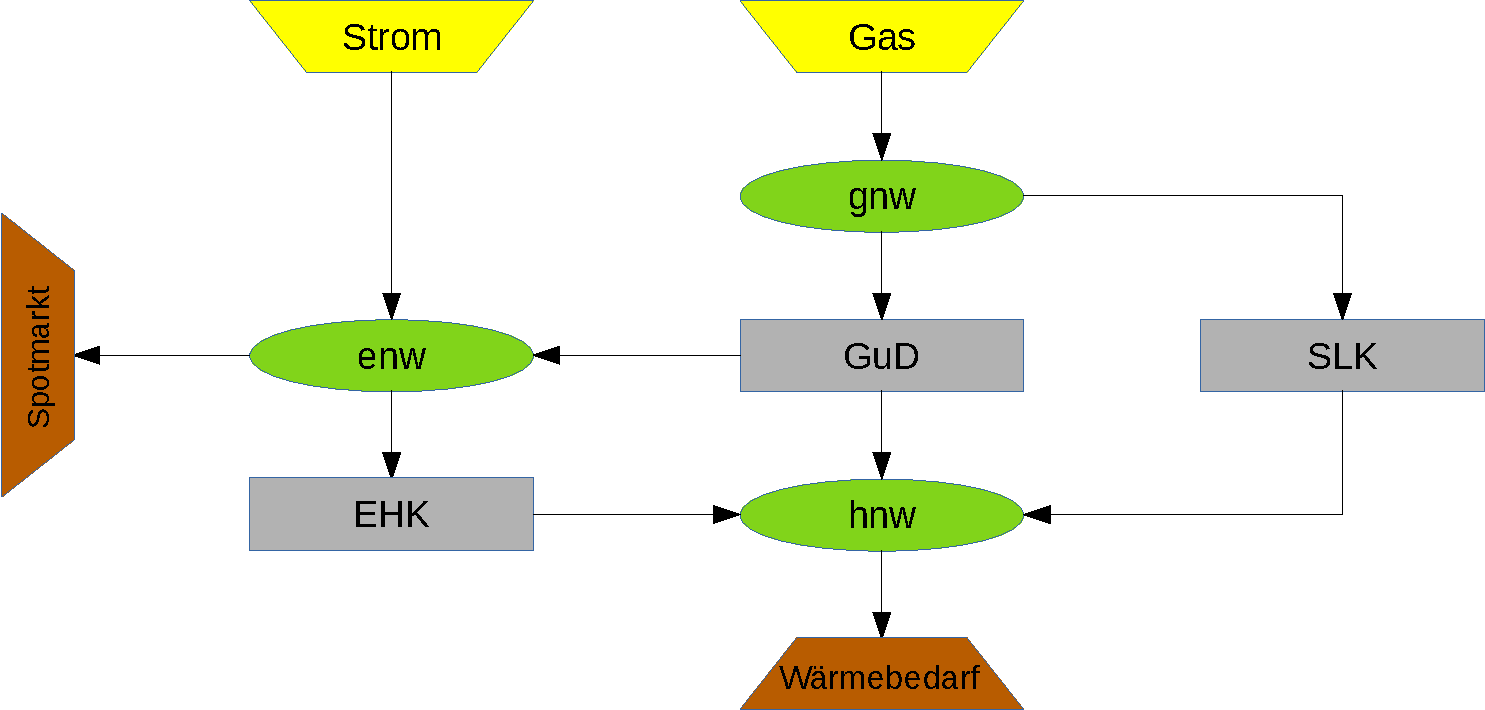
\includegraphics[width=0.8\linewidth]{Solph_Referenzsystem.pdf}
		\captionof{figure}[Schematische Darstellung des in Solph implementierten Referenzsystems]{Schematische Darstellung des in Solph implementierten Referenzsystems. Das benötigte Gas zum Betrieb des \ac{GuD} und \ac{SLK} wird von der Gassource an das Gasnetzwerk (gnw) geliefert. Der \ac{EHK} kann Strom aus dem elektrischen Netz (enw) beziehen, welches aus der Strom-Source und dem \ac{GuD} gespeist wird. Alle Transformer speisen zur Deckung des Wärmebedarfs in das Heiznetzwerk. Bei überschüssiger Stromerzeugung ist eine Vermarktung am Spotmarkt möglich}
		\label{fig: Schema Referenzsystem}
	\end{figure}

Aus dem Datensatz für das Flensburger Fernwärmenetz geht hervor, dass der maximale Wärmebedarf im Jahr 2016 ca. 191,5 MW betrug. Das Referenzsystem ist so dimensioniert, dass eine Reserve von 10 MW vorliegt. Die \ac{GuD}-Anlage soll einen Wärmestrom von bis zu 145 MW liefern. Sowohl der Spitzenlastkessel als auch der Elektrodenheizkessel können maximal 30 MW bereitstellen. Wie in Abbildung \ref{fig: Schema Referenzsystem} zu erkennen ist, beziehen sowohl das \ac{GuD} als auch der \ac{SLK} ihren Brennstoff aus dem Gasnetzwerk (gnw), welches von der Gasquelle gespeist wird. In dem Optimierungsmodell ist der Fluss von der Gasquelle zum Gasnetzwerk mit dem Gaspreis und dem CO$_2$-Zertifikatspreis belegt. Der \ac{EHK} bezieht den elektrischen Strom aus dem eletkrischen Netzwerk (enw) und gibt die Wärme wiederum an das Heiznetzwerk (hnw) ab. Das elektrische Netzwerk wird aus der \ac{GuD}-Anlage und dem eigentlichen Netz versorgt. Der Energiestrom der Strom-Source ist mit der Preiszeitreihe des Day-Ahead-Marktes (im Folgenden Spotmarkt) und den Stromabgaben aus 2016 belegt. Der Energiefluss des \ac{GuD} ist mit den Betriebskosten der Anlage belegt. 

Bei einer Überproduktion an elektrischer Energie kann diese am Spotmarkt zum Preis der Day-Ahead-Auktionen verkauft werden. Hierbei handelt es sich um eine variable Senke, da die Menge an gelieferter Energie nicht festgelegt ist. Im Gegensatz dazu ist der Wärmebedarf an Fernwärme (\ac{DH}) $\dot{Q}^{dh}$ zu jedem Zeitpunkt der Simulation exakt zu decken. Dieser Zusammenhang ist in Gleichung \ref{equation: Bedingung Waermeversorgung} dargestellt:
	\begin{equation}
		\label{equation: Bedingung Waermeversorgung}
		\dot{Q}^{dh} = \dot{Q}_{\text{C}}^{dh} + \dot{Q}_{\text{S}}^{dh} + \dot{Q}_{\text{E}}^{dh}
	\end{equation} 
hierin ist
	\begin{tabbing}
		\hspace{0.5cm}\=\hspace{1cm}\=\hspace{0.5cm}\=\hspace{1cm}\=\kill
		\> $\dot{Q}_{\text{C}}^{dh}$ \>  \>  Wärmestrom des \ac{GuD} an \ac{DH}\\
		\> $\dot{Q}_{\text{S}}^{dh}$ \> \>  Wärmestrom des \ac{SLK} an \ac{DH}\\
		\> $\dot{Q}_{\text{E}}^{dh}$ \> \>  Wärmestrom des \ac{EHK} an \ac{DH}\\
	\end{tabbing} 

Bei der \ac{GuD}-Anlage handelt es sich in Solph um die GenericCHP-Komponente, welche mit den in Kapitel \ref{section: Gas- und Dampfkraftwerk} ermittelten Parametern implementiert worden ist. In Tabelle~\ref{tab: Notwendige Eckdaten zur Verwendung der GenericCHP-Komponente} sind diese Parameter, über die ein zulässiges PQ-Diagramm gebildet wird, bereits aufgeführt worden. Zusätzlich zu diesen Daten ist das \ac{GuD} mit einer Mindest-Standzeit und Startkosten belegt worden, um zu verhindern, dass die Anlage während der Simulation dauerhaft anspringt und nach nur einem Zeitschritt direkt ausgeht. Nach \citet{christidis2011} kann bei einer stündlich aufgelösten Optimierung auf die Modellierung einer Lastrampe beim Start und Stopp des Kraftwerks verzichtet werden. Die Mindest-Standzeit ist mit 5h und die Startkosten mit 4000~$\euro$ in die Simulation eingegangen \cite{christidis2011}. 

Der \ac{EHK} und \ac{SLK} sind als einfache Transformer mit einem konstanten Wirkungsgrad abgebildet worden. Auf eine Mindest-Stillstandzeit und Startkosten wurde bei diesen Komponenten verzichtet. Im Gegensatz zur modellierten \ac{GuD}-Anlage kann der Transformer jeden Betriebspunkt zwischen 0\% und 100\% der Nennleistung  anfahren. Es sind folglich Wärmeströme zwischen 0 und 30~MW von diesen Komponenten zu erwarten. Der \ac{SLK} und \ac{EHK} sind bei der Modellierung möglichst einfach gehalten, um den Simulationsaufwand so weit wie möglich zu reduzieren. 

Ziel der Einsatzoptimierung ist die Minimierung des Betriebsergebnisses, welches, auf Grund der mit negativem Vorzeichen in die Optimierung einfließenden Erlöse für die Fernwärme und Stromvermarktung, negativ ausfällt. Die Zielfunktion, die dieses Modell mathematisch beschreibt, kann Gleichung \ref{equation: Zielfunktion Referenzsystem} entnommen werden:
	\begin{equation}
		\label{equation: Zielfunktion Referenzsystem}
		\text{min }  Z_{Ref} = \text{min} \left[ \sum_{t}^{} \left( (C_{C,t} - R_{C,t}) + (C_{S,t} - R_{S,t}) + (C_{E,t} - R_{E,t}) + C_{CO,t} \right) \right]
	\end{equation}
Sie wird über die Kosten $C$ und Erlöse $R$ der im System verwendeten Technologien gebildet. Wie sich die einzelnen Terme der Zielfunktion zusammensetzen, kann Gleichung \ref{equation: Kosten-GuD} bis \ref{equation: Kosten-CO2} entnommen werden.
	\begin{align}
		\label{equation: Kosten-GuD}
		C_{C,t} &= \dot{Q}_{C,t}^{gas} \cdot  c_{t}^{gas} + P_{C,t} \cdot c_{C,t}^{BK} + Y_{C,t}^{\text{start}} \cdot c_{C,t}^{\text{start}} \\
		R_{C,t} &= \dot{Q}_{C,t}^{dh} \cdot c_t^{dh} + P_{C,t} \cdot c_t^{sm} \\
		C_{S,t} &= \dot{Q}_{S,t}^{gas} \cdot c_{t}^{gas} + \dot{Q}_{S,t}^{dh} \cdot c_{S,t}^{BK} + \dot{Q}_{S,t}^{dh} \cdot c_{S,t}^{es} \\
		R_{S,t} &= \dot{Q}_{S,t}^{dh} \cdot  c_t^{dh} \\
		C_{E,t} &= P_{E,t} \cdot  (c_{t}^{sm} + c_{t}^{sa}) + \dot{Q}_{E,t}^{dh} \cdot c_t^{dh} \\
		R_{E,t} &= \dot{Q}_{E,t}^{dh} \cdot  c_t^{dh} \\
		\label{equation: Kosten-CO2}
		C_{CO2,t} &= \dot{Q}_{gas,t} \cdot  c_{CO2,t}
	\end{align}
Die Kosten des \ac{GuD} $C_{C,t}$ werden über den aufgenommenen Gasstrom $\dot{Q}_{C,t}^{gas}$ und den Gaspreis $c_{t}^{gas}$, die Betriebskosten $c_{C,t}^{BK}$ pro MW elektrischer Leistung $P_{C,t}$ sowie die Startkosten für das Hochfahren der Anlage $c_{C,t}^{\text{start}}$ gebildet. Entsprechend wird der Erlös in Gleichung \ref{equation: Kosten-CO2} über die erzeugte Fernwärme und die vermarktete elektrische Leistung gebildet. Analog werden die anderen Technologien beschrieben. Die Kosten der CO$_2$-Zertifikate werden über den gesamten Gasstrom zum Zeitpunkt $t$ und den Zertifikatspreis $c_{CO2,t}$ abgebildet.
Die Bedeutung der verwendeten Indizes und Abkürzungen kann folgender Auflistung entnommen werden.

	\begin{tabular}{llllll}
		&&&&&  \tabularnewline
		C & \acl{GuD} & es & Energiesteuer & Y & Statusvariable Ein/Aus\tabularnewline
		&&&&& \tabularnewline
		S & \acl{SLK} & BK & Betriebskosten & start & Startbezug\tabularnewline
		&&&&& \tabularnewline
		E & \acl{EHK} & sm & Spotmarkt & $t$ & Zeitschritt \tabularnewline
		&&&&&  \tabularnewline
		&  & sa & Stromabgaben &  & \tabularnewline
	\end{tabular}

\section{Alternativsysteme}
Bei den Alternativsystemen handelt es sich stets um das bereits beschriebene Referenzsystem, welches um die in Kapitel \ref{section: Konzepte} ausgewählten Konzepte der solarthermischen Wärmebereitstellung erweitert wurde. Die Anlagendimensionierung des Referenzsystems hat sich bei der Erweiterung um andere Technologien nicht geändert. Das heißt, dass die mögliche Überproduktion an Wärme im Vergleich zum Referenzsystem steigt. Die Alternativsysteme, welche in den folgenden Abschnitten genauer betrachtet werden, sind mit drei verschiedenen Anlagengrößen für die Solarthermie und den Saisonalen Speicher simuliert worden. Danach ergeben sich für jedes Konzept insgesamt neun verschiedene Setups. Folgende Anlagendimensionierungen wurden betrachtet:

	\begin{tabular}{llllll}
		&&&&&  \tabularnewline
		\textbf{Kollektorfläche:} & 70.000 & \textbf{140.000} & 210.000 & m$^2$  \tabularnewline
		&&&&& \tabularnewline
		\textbf{Speicherkapazität:} & 20.000 & \textbf{60.000} & 100.000 & MWh \tabularnewline
		&&&&& \tabularnewline	
	\end{tabular}

In der Auflistung ist eine Kollektorfläche von 140.000~m$^2$ und eine Speicherkapazität des \ac{STES} von 60 GWh hervorgehoben worden, da diese Auslegungen für die Alternativsysteme als Basis-Szenario festgelegt wurden. Die Kollektorfläche ist vor dem Hintergrund gewählt worden, dass der Solaranlagen-Ertrag am sonnigsten Tag des Jahres (nach vorliegendem Datensatz der 11.06.) gleich dem Wärmebedarf dieses Tages sein soll. Die daraus hervorgehende Fläche von 140.000~m$^2$ liegt nur knapp unter der derzeit größten Anlage in Silkeborg, die eine Fläche von 156.694~m$^2$ aufweist \cite{SDH2019}. Bei der Speichergröße ist die Anlage in Vojens als Vorlage für das Basis-Szenario verwendet worden, welche über ein Speichervolumen von 200.000~m$^3$ verfügt \cite{Arcon2019}. Bei einer maximalen Energiedichte von 300~kWh/m$^3$ \cite{Sterner2017} entspricht dies einer Kapazität von 60~GWh. Das Basis-Szenario dient als Ausgangspunkt für bei der Berechnung der Kostendegression des \ac{STES}.

\subsection{Solarthermie 1}\label{subsection: Solarthermie 1}
Bei dem Solarthermie 1-Konzept (ST1), welches in Abbildung \ref{fig: Solph_Solarthermie_1} dargestellt wird, handelt es sich um das Referenzsystem, welches um eine Solarthermieanlage und einen saisonalen Wärmespeicher erweitert worden ist. Der spezifische Ertrag (MW/m$^2$) der Solaranlage ist im Preprocessing über die DIN EN 12975 und die in Kapitel \ref{section: Modellbildung - Solarthermie} ermittelten Verlustparameter für Kollektorfelder - bestehend aus Vakuumröhrenkollektoren - bestimmt worden. Dieser ist als Datenreihe an das Optimierungsmodell übergeben worden und wird in diesem als Source abgebildet, die direkt mit dem Heiznetzwerk verbunden ist. Je nach Anlagengröße ist dieser Eingang entsprechend skaliert worden. Es ist davon ausgegangen worden, dass durch den \ac{STES} 100\% der solaren Wärme abgenommen werden kann, weshalb die Solar-Source als fixe Eingangsgröße modelliert worden ist. D. h., dass der Ertrag der Solaranlage auf jeden Fall abgenommen werden muss. Dies gilt entsprechend für alle untersuchten Konzepte.
	\begin{figure}[ht]
		\centering
		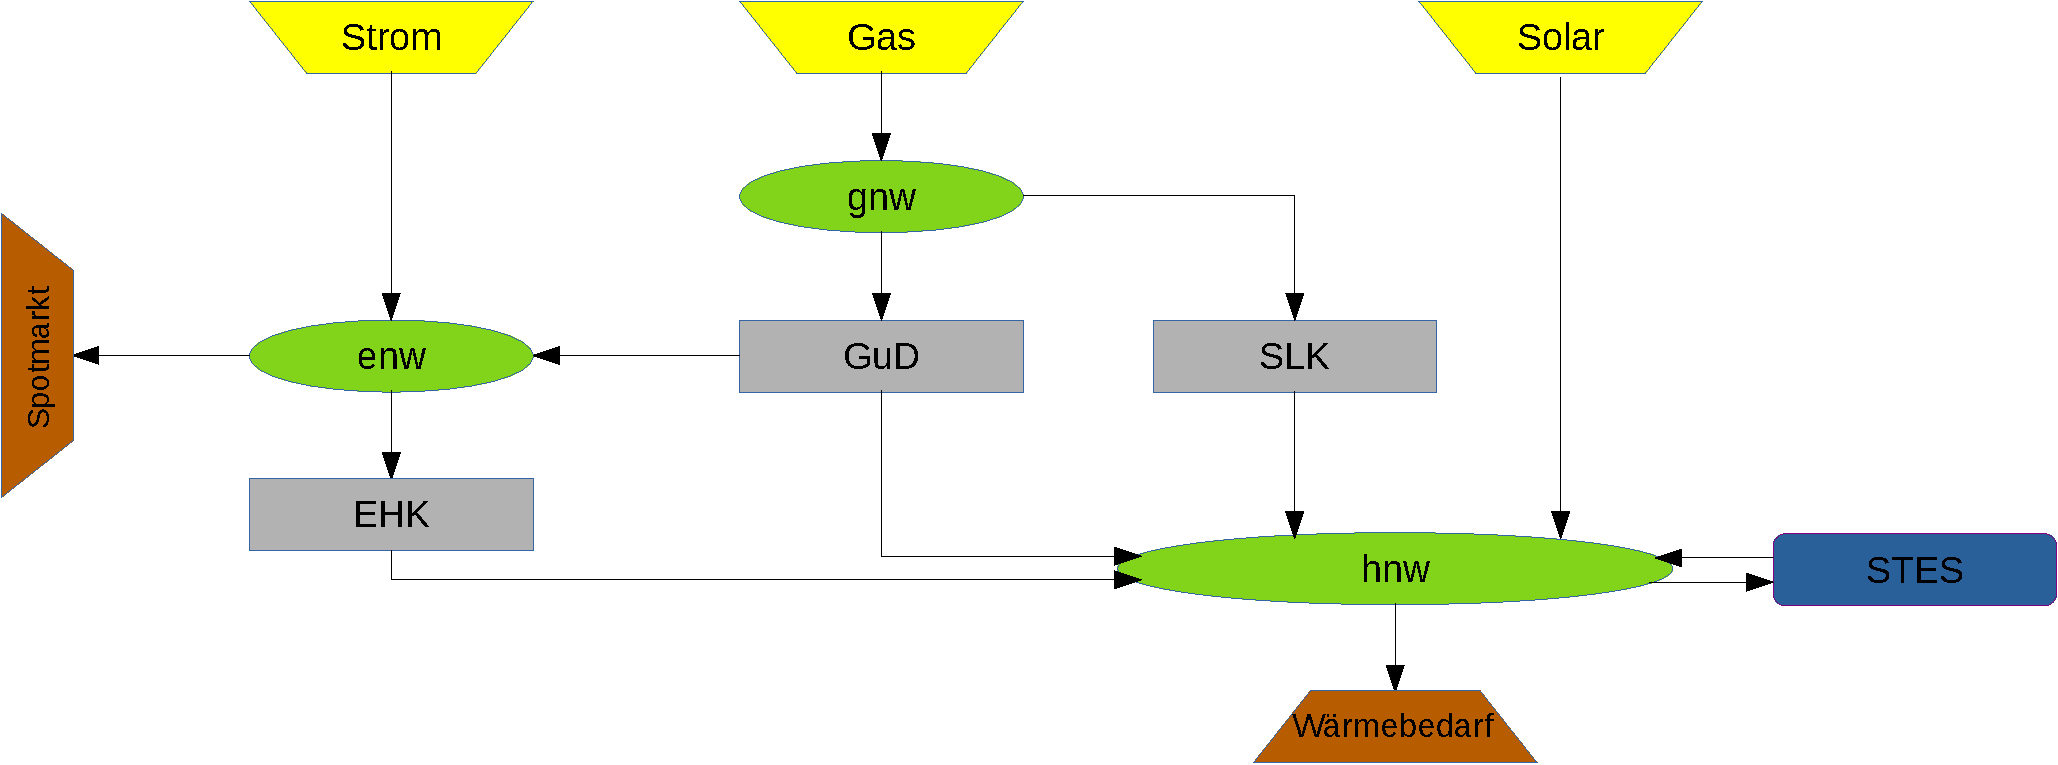
\includegraphics[width=0.8\linewidth]{Solph_Solarthermie_1.pdf}
		\captionof{figure}[Schematische Darstellung des in Solph implementierten Solarthermie 1-Konzepts]{Dargestellt wird eine schematische Darstellung des in Solph implementierten Solarthermie 1-Konzepts. Dabei handelt es sich um das Referenzsystem welches um eine Solar-Source und einen \ac{STES} erweitert worden ist. Der Ertrag aus der Solarthermie ist, wie der \ac{STES} auch, direkt an das hnw angeschlossen.}
		\label{fig: Solph_Solarthermie_1}
	\end{figure}

Tabelle \ref{tabelle: Übersicht flächenspezifische Daten} zeigt, abhängig von der Fläche, den im Preprocessing berechneten Ertrag, die \ac{SF}, Investitionskosten und die Betriebskosten der Solaranlage, welche in der Optimierung mit berücksichtigt werden. Die \ac{SF} stellt hier den maximal möglichen Wert dar, sollte die Wärme aus der Solarthermie ausschließlich direkt genutzt und nicht zwischengespeichert werden, da die Speicherung verlustbehaftet ist. 
	\begin{center}
		\captionof{table}{Übersicht über flächenspezifische Daten der Solarthermie-Anlage}
		\label{tabelle: Übersicht flächenspezifische Daten}
		\begin{tabular}{ccccc}
			\hline 
			Fläche [m$^2$] & Ertrag [MWh] & \ac{SF} [\%] & Investition [\euro]  & Betriebskosten [\euro/MWh] \tabularnewline
			\hline 
			70.000 & 33.331 & 5,57 & 19.135.308 & 5,74 \tabularnewline
			140.000 & 66.622 & 11,14 & 34.327.855 & 5,15 \tabularnewline
			210.000 & 99.933 & 16,71 & 48.032.234 & 4,81 \tabularnewline		
			\hline
		\end{tabular}
	\end{center} 

Der von der Solaranlage übers Jahr maximal abgegebene Wärmestrom ist für den \ac{STES} als höchstmöglicher Wärmeeingang zum Aufladen des Speichers festgelegt worden. Dieser Wert variiert entsprechend der Kollektorfläche. Ein maximaler Entlade-Wärmestrom ist hingegen wesentlich höher angesetzt. Es soll möglich sein, das Wärmenetz zu 100\% aus dem Speicher versorgen zu können, weshalb die Entladung maximal mit der höchstmöglichen Last des Netzes erfolgen kann - in diesem Fall mit 191,5 MW. Darüber hinaus ist der Speicherwirkungsgrad von 75\% auf den abgegebenen Wärmestrom bezogen. Um zu verhindern, dass der Saisonale Speicher wie ein Kurzzeitspeicher genutzt wird, der stündlich aus- und entladen wird, ist der \ac{STES} mit einer minimalen Auflade- und Entladezeit von 3h modelliert worden. Darüber hinaus ist der Speicherstand zu Beginn des betrachteten Zeitraums auf 70\% seiner Kapazität festgelegt. Die kapazitätspezifischen Betriebskosten des Speichers können Tabelle \ref{tabelle: Übersicht kapazitätsspezifische Daten} entnommen werden.
	\begin{center}
		\captionof{table}{Übersicht über kapazitätspezifische Daten des saisonalen thermischen Energiespeichers} 
		\label{tabelle: Übersicht kapazitätsspezifische Daten}
		\begin{tabular}{ccccc}
			\hline 
			Kapazität [GWh] &  &  & Investition (mit Förderung) [\euro]  & Betriebskosten [\euro/MWh] \tabularnewline
			\hline 
			20 &  &  & 7.966.141 & 0.66 \tabularnewline
			60 &  &  & 15.400.000 & 0.43 \tabularnewline
			100 &  &  & 20.923.290 & 0.35 \tabularnewline		
			\hline
		\end{tabular}
	\end{center}

Mathematisch kann die Zielfunktion des ST1-Modells analog zum Referenzsystem beschrieben werden. Sie muss lediglich um einen Term für die Solarthermie-Anlage (ST) und den \ac{STES} erweitert werden. Dies ist in Gleichung \ref{equation: Zielfunktion ST 1} dargestellt.
\begin{equation}
	\label{equation: Zielfunktion ST 1}
	\text{min } Z_{\text{ST1}} = \text{min} \left[Z_{\text{Ref}} +  \sum_{\text{t}}^{} \left((C_{\text{ST,t}} - R_{\text{ST,t}}) + C_{\text{STES,t}} \right)   \right]
\end{equation}
Wie sich die Kosten und der Erlös der Solarthermie-Anlage sowie die Kosten des Speichers bilden, ist Gleichung \ref{equation: Kosten-ST} bis \ref{equation: Kosten_STES} zu entnehmen.
\begin{align}
	\label{equation: Kosten-ST}
	C_{\text{ST,t}} &= \dot{Q}_{\text{ST,t}}^{\text{DH}} \cdot c_{\text{ST,t}}^{\text{BK}} \\
	R_{\text{ST,t}} &= \dot{Q}_{\text{ST,t}}^{\text{DH}} \cdot c_{\text{t}}^{\text{DH}}\\
	\label{equation: Kosten_STES}
	C_{\text{STES,t}} &= \dot{Q}_{\text{STES,t}}^{\text{ein}} \cdot c_{\text{STES,t}}^{\text{BK}}
\end{align}


\subsection{Solarthermie 2}
Abbildung \ref{figure: Solph_Solarthermie_2} zeigt das Solarthermie 2-Konzept (ST2) in der Form, wie es in Solph implementiert worden ist. Es wurden zusätzlich zur solarthermischen Anlage und dem \ac{STES} des ST1-Konzepts eine Wärmepumpe und ein Kurzzeitspeicher hinzugefügt.
	\begin{figure}[ht]
		\centering
		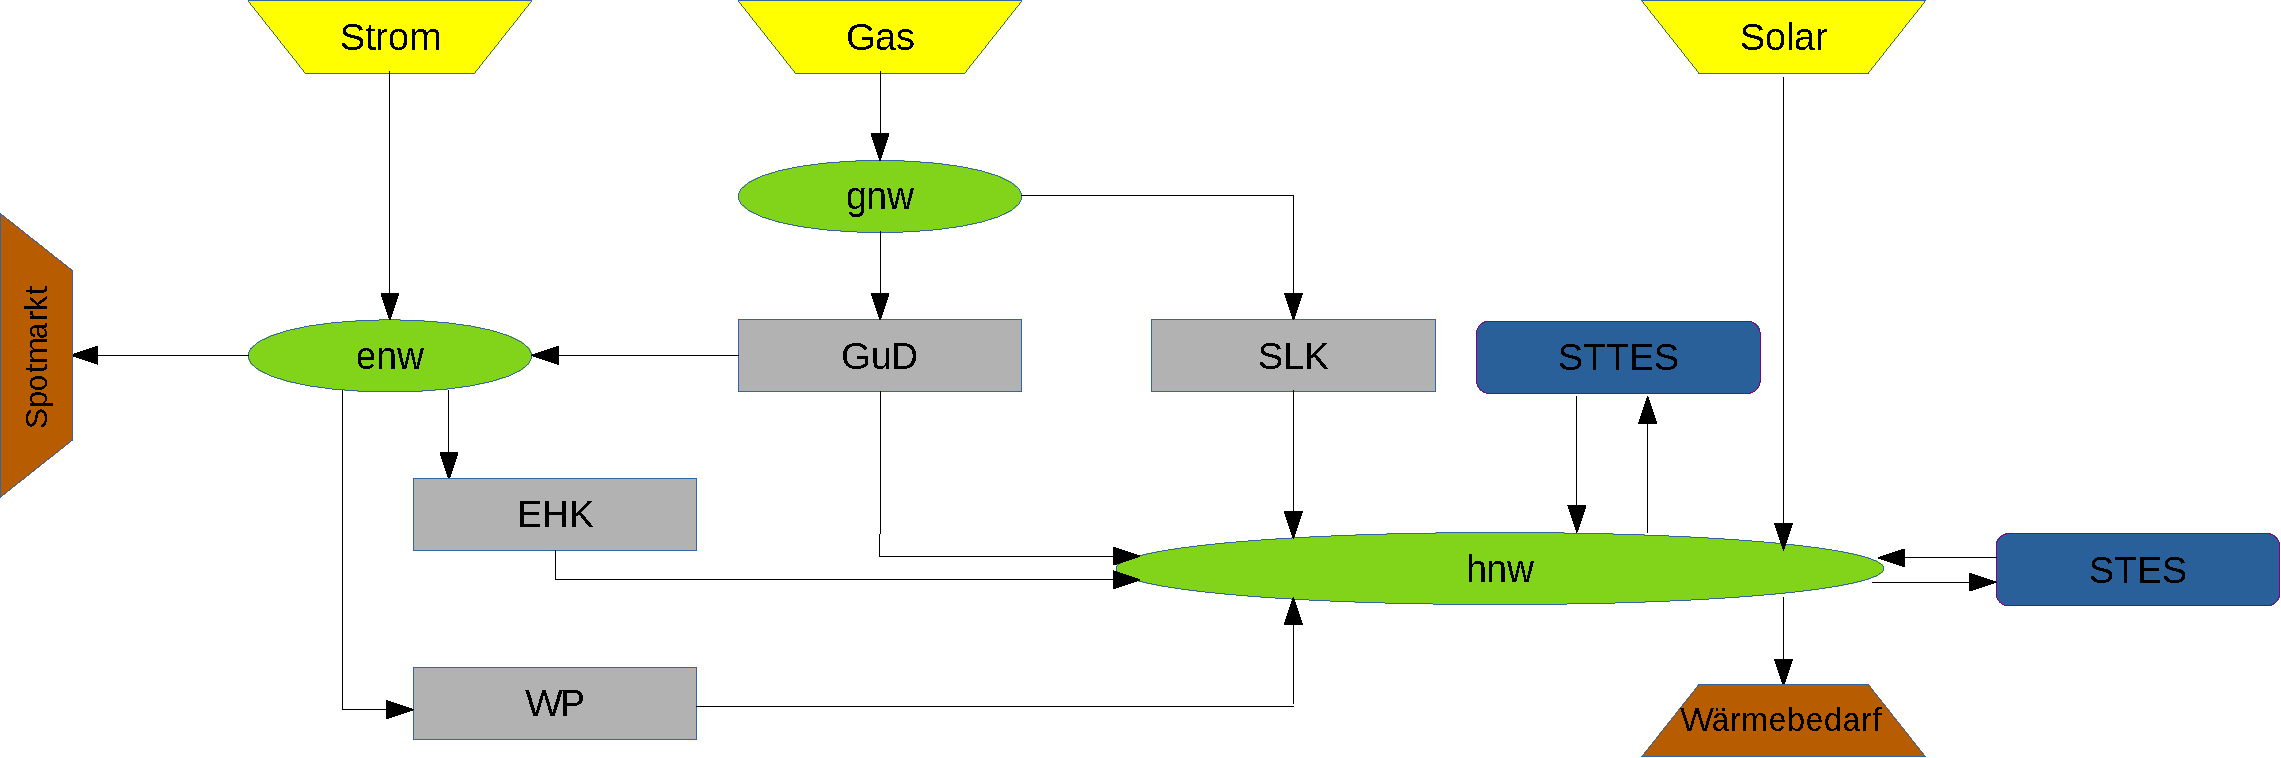
\includegraphics[width=0.8\linewidth]{Solph_Solarthermie_2.pdf}
		\captionof{figure}[Schematische Darstellung des in Solph implementierten Solarthermie 2-Konzepts]{Schematische Darstellung des in Solph implementierten Solarthermie 2-Konzepts. Hierbei handelt es sich um das ST1-Konzept, welches um einen Kurzzeitspeicher und eine Wärmepumpe erweitert wurde. Der Speicher (STTES) ist direkt mit dem hnw verbunden - die Wärmepumpe bezieht den elektrischen Strom aus dem enw und speist die Wärme in hnw.}
		\label{figure: Solph_Solarthermie_2}
	\end{figure}

Die Wärmepumpe ist in Solph als OffsetTransformer modelliert worden. Das heißt, dass die \ac{WP} in dieser Optimierung unter einer Leistung von 40\% ihrer Nennleistung nicht arbeitet. Über die \ac{TESPy}-Simulation einer Wärmepumpe ist, wie in Kapitel \ref{section: Modellbildung - Kompressionswärmepumpe} bereits dargestellt, der Gütegrad über einer variierenden Auslastung ermittelt worden. Dieser ist genutzt worden, um die linearisierte Rampe des OffsetTransformers zu definieren. Zusammen mit der, im Preprocessing ermittelten, Carnot-Leistungszahl, die als Datenreihe an das Optimierungsmodell übergeben wird, ist für jeden Zeitschritt eine Leistungs- und Temperaturabhängigkeit (Umgebung und Vorlauf des Netzes) realisiert worden.

Die Kapazität des Kurzzeitspeichers ist so gewählt worden, dass er theoretisch den Wärmebedarf des Netzes über 6~Stunden decken kann. Bei einem maximalen Bedarf von 191,5~MW entspricht dies einer Kapazität von 1149~MWh. Die Idee hinter der Verwendung des Kurzzeitspeichers ist, den Einsatz der Wärmepumpe zu optimieren - Wärmeproduktion bei niedrigen Strompreisen und zwischenspeichern im Kurzzeitspeicher - ist der maximale Be- und Entladewärmestrom des Speichers auf die \ac{WP} abgestimmt, dessen maximal bereitgestellte Wärme vor der Einsatzoptimierung auf 40~MW abgeschätzt worden ist. Entsprechend wurde dieser Wert für die maximale Be- und Entladung des Speichers übernommen. Im Gegensatz zum \ac{STES} ist beim Kurzzeitspeicher kein Speicherstand zu Beginn der Optimierung vorgegeben worden - dieser ist ein Ergebnis der Einsatzoptimierung. Analog zur \ac{WP} ist die Auslegung des Kurzzeitspeichers Szenario unabhängig. 

Um die mathematische Beschreibung der Zielfunktion des ST2-Konzepts zu erhalten ist die ST1-Funktion um einen Term für die Wärmepumpe und den Kurzzeitspeicher zu erweitern. Dies wird in Gleichung \ref{equation: Zielfunktion ST 2} dargestellt. Gleichung \ref{equation: Kosten-WP} bis \ref{equation: Kosten_STTES} beschreiben dabei die Kosten $C_\text{WP,t}$ und den Erlös $R_\text{WP,t}$ der Wärmepumpe sowie die Kosten des Kurzzeitspeichers $C_{\text{STTES,t}}$.
	\begin{equation}
		\label{equation: Zielfunktion ST 2}
		\text{min } Z_\text{ST2} = \text{min} \left[Z_\text{ST1} + \sum_{\text{t}}^{} ((C_\text{WP,t} - R_\text{WP,t}) + C_\text{STTES,t}) \right]
	\end{equation}
	\begin{align}
		\label{equation: Kosten-WP}
		C_\text{WP,t} &= \dot{Q}_\text{WP,t}^\text{DH} \cdot c_\text{WP,t}^\text{BK} + P_\text{WP,t} (c_\text{t}^\text{sm} + c_\text{t}^\text{sa}) \\
		R_\text{WP,t} &= \dot{Q}_\text{WP,t}^\text{DH} \cdot c_\text{t}^\text{DH}\\
		\label{equation: Kosten_STTES}
		C_{\text{STTES,t}} &= \dot{Q}_{\text{STTES,t}}^{\text{ein}} \cdot c_\text{STTES,t}^\text{BK}
	\end{align}

\subsection{Photovoltaik}
Im Gegensatz zu den vorangegangenen Konzepten, wie in Kapitel \ref{subsection: Konzepte - Photovoltaik und Wärmepumpe} bereits beschrieben, handelt es sich bei diesem Konzept um ein indirektes Solarthermie Konzept bei dem die Wärme nicht direkt von solarthermischen Kollektoren bereitgestellt wird. Zunächst stellen \ac{PV}-Module dem enw elektrischen Strom zur Verfügung, welcher von Wärmepumpen zur Wärmebereitstellung genutzt werden kann. Darüber hinaus ist es jedoch auch möglich den gewonnen \ac{PV}-Strom direkt am Spotmarkt zu vermarkten. Ebenso kann die Wärmepumpe betrieben werden, wenn keine Sonneneinstrahlung vorhanden ist - in diesem Fall wird sie über das \ac{GuD} oder aus dem Strommarkt versorgt. Das in Solph modellierte Energiesystem kann Abbildung \ref{figure: Solph_Photovoltaik} entnommen werden.
	\begin{figure}[ht]
		\centering
		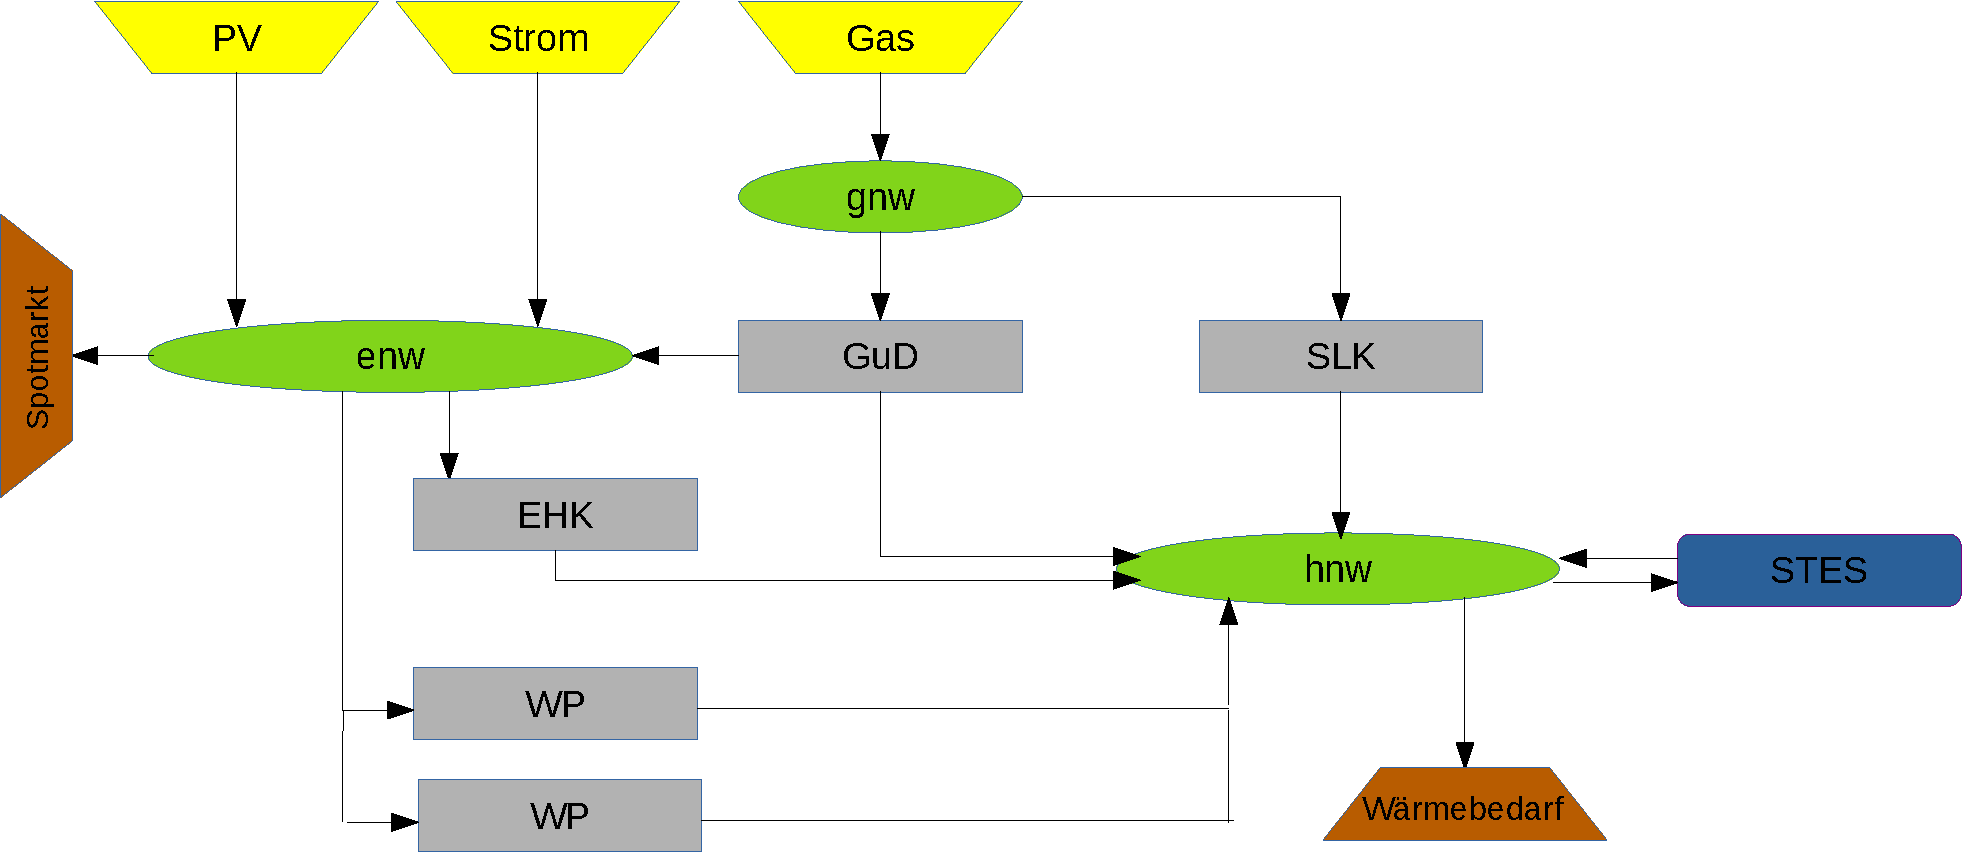
\includegraphics[width=0.8\linewidth]{Solph_Photovoltaik.pdf}
		\captionof{figure}[Schematische Darstellung des in Solph modellierten Photovoltaik-Konzepts]{Schematische Darstellung des in Solph modellierten Photovoltaik-Konzepts. Die von der \ac{PV}-Anlage bereitgestellte elektrische Leistung wird direkt ans enw geliefert, an das auch die beiden Wärmepumpen angeschlossen sind, die den \ac{PV}-Strom zu Bereitstellung von Wärme nutzen können.}
		\label{figure: Solph_Photovoltaik}
	\end{figure}

Der spezifische Ertrag der \ac{PV}-Module ist im Preprocessing über Gleichung \ref{equation: LeistungPV} bestimmt worden und wird als Datenreihe an das Optimierungsmodell übergeben. In dem Modell wird der \ac{PV}-Strom als Source abgebildet und ist an das enw angeschlossen. Entsprechend des Szenarios ist dieser Eingang skaliert worden. Tabelle \ref{tabelle: Übersicht flächenspezifische Daten PV} kann abhängig von dem betrachteten Szenario der Ertrag, die Investitionskosten und Betriebskosten der \ac{PV}-Anlage entnommen werden. 
	\begin{center}
		\captionof{table}{Übersicht über flächenspezifische Daten des Photovoltaik-Konzepts}
		\label{tabelle: Übersicht flächenspezifische Daten PV}
		\begin{tabular}{ccccc}
			\hline 
			Fläche [m$^2$] & Ertrag [MWh] & & Investition [\euro]  & Betriebskosten [\euro/MWh] \tabularnewline
			\hline 
			70.000 & 11.591 & & 11.101.514 & 9,58 \tabularnewline
			140.000 & 23.181 & & 16.826.748 & 7,26 \tabularnewline
			210.000 & 99.933 & & 21.461.247 & 6,17 \tabularnewline		
			\hline
		\end{tabular}
	\end{center} 

Um mit Sicherheit 100\% des \ac{PV}-Stroms in Wärme umwandeln zu können sind zwei Wärmepumpen, die identisch zu der bereits im ST2-Konzept beschriebenen \ac{WP} sind, verwendet worden - diese Anzahl bleibt in jedem Szenario gleich. 
Der \ac{STES} unterscheidet sich in der Modellierung ebenfalls nicht von den vorangegangenen Szenarien. Dementsprechend kann eine genauere Beschreibung der Speicher-Modellierung sowie die von der Kapazität abhängigen Betriebskosten Kapitel \ref{subsection: Solarthermie 1} entnommen werden. 

Die Zielfunktion des Photovoltaik Konzepts ist durch Ergänzung der Referenzsystem-Funktion mit Termen für die \ac{PV}-Anlage, die \ac{WP} und den \ac{STES} zu erhalten - dargestellt in Gleichung \ref{equation: Zielfunktion PV}. Aufgrund der Tatsache, dass in diesem Konzept mehrere Wärmepumpen verwendet werden, sind die Kosten hierfür in allgemeiner Form für eine beliebige Anzahl formuliert worden.
	\begin{equation}
		\label{equation: Zielfunktion PV}
			\text{min } Z_\text{PV} = \text{min} \left[Z_\text{Ref} + \sum_{\text{t}}^{} \left( \sum_\text{\text{WP}}^{} (C_\text{WP,t} - R_\text{WP,t}) + (C_\text{PV,t} - R_\text{PV,t}) + C_\text{STES,t}  \right)     \right]
	\end{equation}

In Gleichung \ref{equation: WP-PV} bis \ref{equation: ErlösPV} wird gezeigt wie sich die einzelnen Terme zusammensetzen. Die Kosten der \ac{WP} bilden sich beispielsweise über den abgegebenen Wärmestrom und die Betriebskosten sowie über die elektrische Leistung und die Summe aus dem Strompreis und den Stromabgaben. 
	\begin{align}
		\label{equation: WP-PV}
		C_\text{WP,t} &= \dot{Q}_\text{WP,t}^\text{DH} \cdot c_\text{WP,t}^\text{BK} + P_\text{WP,t} (c_\text{t}^\text{sm} + c_\text{t}^\text{sa})\\
		R_\text{WP,t} &= \dot{Q}_\text{WP,t}^\text{DH} \cdot c_\text{t}^\text{DH}\\
		C_\text{PV,t} &= \dot{P}_\text{PV,t}^\text{sm} \cdot c_\text{PV,t}^\text{BK} \\
		\label{equation: ErlösPV}\text{}
		R_\text{PV,t} &= \dot{P}_\text{PV,t}^\text{sm} \cdot c_\text{t}^\text{sm}
	\end{align}


\section{Ergebnisse der Einsatzoptimierung}
Nach der Vorstellung aller betrachteten Konzepte in den vorangegangenen Abschnitten wird dieser Abschnitt die Ergebnisse der Einsatzoptimierungen, die mit dem Ziel der Erlös-Optimierung durchgeführt worden sind, für das Referenzsystem und die Alternativsysteme vorstellen. Dabei steht zunächst die Frage im Vordergrund, wie wirtschaftlich die verschiedenen Konzepte und Szenarien im Vergleich zum Referenzsystem sind. Zu diesem Zweck ist vorerst der Kapitalwert genutzt worden. Für die jeweils aussichtsreichsten Auslegungen werden genauere Untersuchung des Betriebsverhaltens der einzelnen Komponenten durchgeführt.

\subsection{Ergebnis der Einsatzoptimierung des Referenzsystems} 
Das Referenzsystem dient als Vergleich zu den erstellten Solarthermie-Systemen und wird zur ökonomischen Bewertung der untersuchten Alternativsysteme herangezogen. Die Einsatzoptimierung des Referenzsystems hat einen, beim optimalen Betrieb der Anlagen, möglichen Erlös von 44,38~Mio.~\euro/a ergeben. Dieser Erlös setzt sich aus der Differenz zwischen den Kosten zum Betrieb der Anlage und Einnahmen durch den Verkauf von Strom und Wärme zusammen. Insgesamt konnte durch die Bereitstellung von Wärme ein Betrag von 41,04~Mio.~\euro\ eingenommen werden. Dieser Wert ist aufgrund eines konstanten Wärmepreises und des gleichbleibenden Wärmebedarfs bei jedem Konzept/Szenario identisch. Die Einnahmen aus dem Verkauf von Strom am Spotmarkt belaufen sich auf 73,9~Mio.~\euro\ und sind damit knapp 80\% größer als die Einnahmen durch den Verkauf von Wärme. Der Kapitalwert des Referenzsystems beträgt, bei einer angenommenen Laufzeit von 20 Jahren und einer Verzinsung von 5\%, insgesamt 267,57~Mio.~\euro. Die Kapitalwerte der Alternativsysteme werden auf diesen Referenz-Kapitalwert bezogen und zeigen somit bei positiven Werten an, dass das Konzept wirtschaftlich attraktiver ist, als das einfache Referenzsystem. Entsprechend zeigen negative Kapitalwerte (bezogen auf das Referenzsystem) an, dass es wirtschaftlicher ist, das Referenzkonzept zu betreiben, ohne die Einbringung von Solarthermie.

	\begin{figure}[ht]
		\centering
		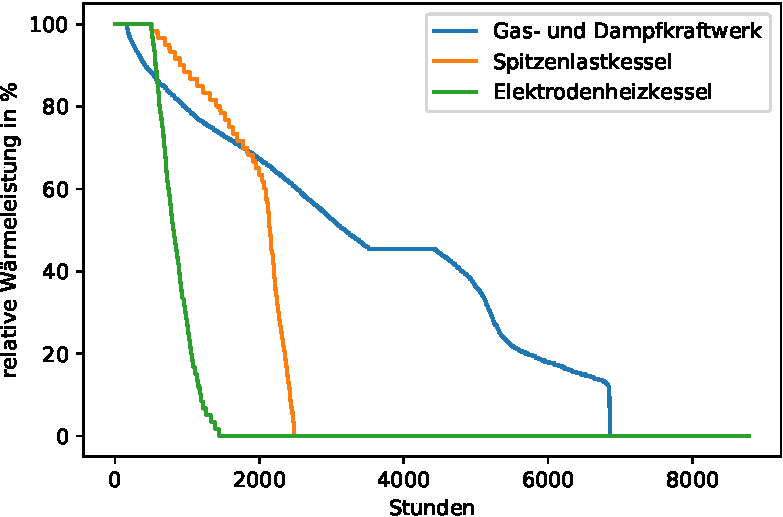
\includegraphics[width=0.8\linewidth]{Jahresdauerlinie_Referenzsystem-cropped.pdf}
		\captionof{figure}[Jahresdauerlinien des Referenzsystems]{Jahresdauerlinien der Wärmebereitstellung aller verwendeten Technologien innerhalb des Referenzsystems. Auf der Abszisse sind die Stunden des Jahres aufgetragen - die Ordinate zeigt die relative Wärmeleistung.}
		\label{figure: Jahresdauerlinien_Referenzsystem}
	\end{figure}

Um das Anlagenverhalten zwischen den Konzepten besser vergleichen zu können ist eine Darstellung des Betriebes in Jahresdauerlinien gewählt worden. Dieser Darstellungsform ist direkt, unabhängig von der entsprechenden Leistung, zu entnehmen, wie eine Anlage über das Jahr betrieben worden ist. Der abgegebene Wärmestrom der Anlage wird in dieser Darstellung auf den über das betrachtete Jahr maximal auftretenden Wärmestrom bezogen. Somit lässt sich Abbildung \ref{figure: Jahresdauerlinien_Referenzsystem} direkt entnehmen, wie viele Stunden die Anlage betrieben worden ist und wie groß der Teillast-Anteil ist.

Es ist zu erkennen, dass die \ac{GuD}-Anlage mit 6850~Betriebsstunden die bevorzugte Technologie zur Wärmebereitstellung darstellt. Es ist aber auch zu erkennen, dass das \ac{GuD} in diesem System nur für wenige Stunden im Jahr ihren vollen Wärmestrom abgibt und quasi dauerhaft in Teillast Wärme bereitstellt. Das heißt jedoch nicht, dass das \ac{GuD} generell in Teillast betrieben wird, da das modellierte Kraftwerk 2 Freiheitsgrade und die Bereitstellung von Wärme und Strom somit entkoppelt sind. Bezogen auf die abgegebene elektrische Energie erreicht das Kraftwerk eine Volllaststundenzahl für den betrachteten Zeitraum von 5371~h. 

Bei dem Betrieb des \ac{EHK} und \ac{SLK} ist zu erkennen, dass diese mit knapp 1500 und 2500~Betriebsstunden deutlich weniger genutzt werden als die \ac{GuD}-Anlage. Beide Anlagen werden unter Volllast über ungefähr den gleichen Zeitraum  verwendet. Die Jahresdauerlinie des Elektrodenheizkessels fällt im Vergleich zum Spitzenlastkessel jedoch stark ab - im niedrigen Leistungsbereich wird der \ac{EHK} nur wenig genutzt. Hervorgehoben wird in Abbildung \ref{figure: Jahresdauerlinien_Referenzsystem} die Bedeutung des \ac{SLK} in dem Referenzsystem. Nach dem \ac{GuD} ist der \ac{EHK} deutlich häufiger und mit einer höheren Auslastung als der \ac{EHK} verwendet worden. Überwiegend ist der Spitzenlastkessel in einem Leistungsbereich zwischen 60\% und 100\% eingesetzt worden. Insgesamt werden im Referenzsystem 86,15\% des Wärmebedarfs von dem \ac{GuD} gedeckt. Der \ac{SLK} stellt 9,6\% und der \ac{EHK} 4,25\% des gesamten Wärmebedarf zur Verfügung. Diese Zahlen heben noch einmal deutlich die Rolle der \ac{GuD}-Anlage im Referenzsystem hervor. 

Die Wärmegestehungskosten des Referenzsystems werden nach Gleichung \ref{equation: vereinfacht Wärmegestehung} berechnet und betragen 32,7 \euro/MWh. Dieser Wert liegt ungefähr in der selben Größenordnung der Wärmegestehungskosten eines auf fossilen Energieträgern basierten Konzepts, bestehend aus einem Blockheizkraftwerk, einer Gegendruckturbine sowie einem Spitzenlast- und Elektrodenheizkessel, welches von \citet{Kaldemeyer2019} untersucht worden ist. Das Ergebnis der Optimierung wird somit als plausibel angesehen.

\subsection{Ergebnisse der Einsatzoptimierung der Alternativsysteme}
An dieser Stelle wird zunächst entschieden, welche Szenarien der einzelnen Konzepte genauer untersucht werden sollen. Als Entscheidungsvariable wird an dieser Stelle der Kapitalwert verwendet. Er wird über die Differenz des Betriebsergebnisses der Alternativkonzepte und dem Ergebnis des Referenzsystems gebildet. In Anlehnung an Gleichung \ref{equation: Kapitalwert-vereinfact} wird die Differenz zwischen den Einnahmen und Ausgaben $(E - A)$ nach Gleichung \ref{equation: E-A} berechnet. Die Investitionskosten beziehen sich bei dieser Rechnung auf die Investitionen, welche das Referenzsystem erweitern.
	\begin{equation}
	\label{equation: E-A}
		(E - A) = (E - A)_\text{Alternativsystem} - (E - A)_\text{Referenzsystem}
	\end{equation}

Abbildung \ref{fig: Heatmaps Solarthermie} und \ref{figure: Heatmap Photovoltaik} zeigen die Ergebnisse der Kapitalwertberechnung für die beiden Solarthermie-Konzepte und das Photovoltaik-Konzept in Form einer Heatmap. Darin werden die Szenarien mit hohen Kapitalwerten dunkel und diejenigen mit niedrigen Werten hell eingefärbt. Diese Heatmaps werden in diesem Abschnitt genutzt, um die Ergebnisse der unterschiedlichen Szenarien zu bewerten.
	\begin{figure}
		\begin{subfigure}[b]{0.48\textwidth}
			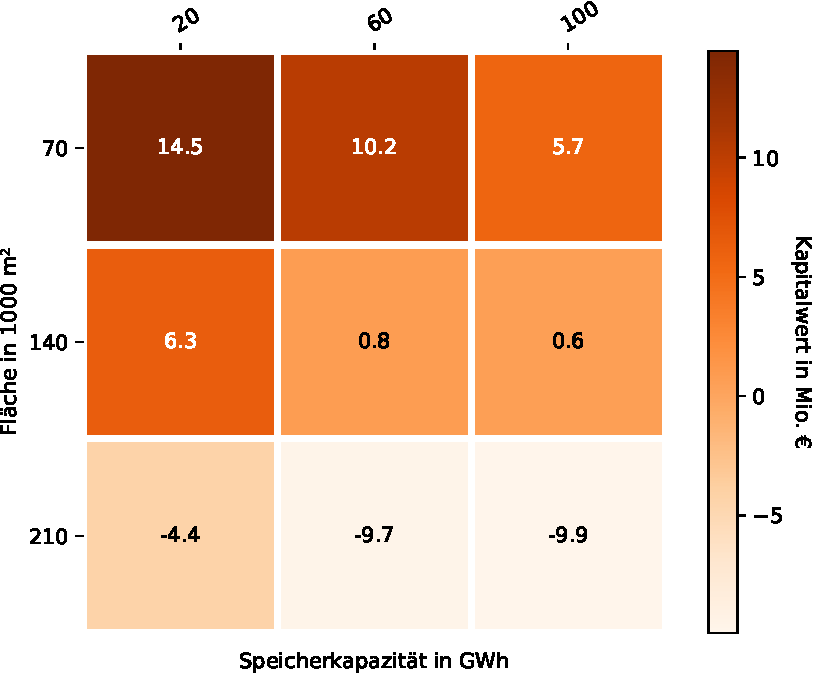
\includegraphics[width=1\textwidth]{Verbesserung/Solar1_Heatmap_relNPV-cropped.pdf}
			\subcaption{Solarthermie 1}
			\label{fig: Heatmaps Solarthermie a}
		\end{subfigure}
		\hfill
		\begin{subfigure}[b]{0.48\textwidth}
			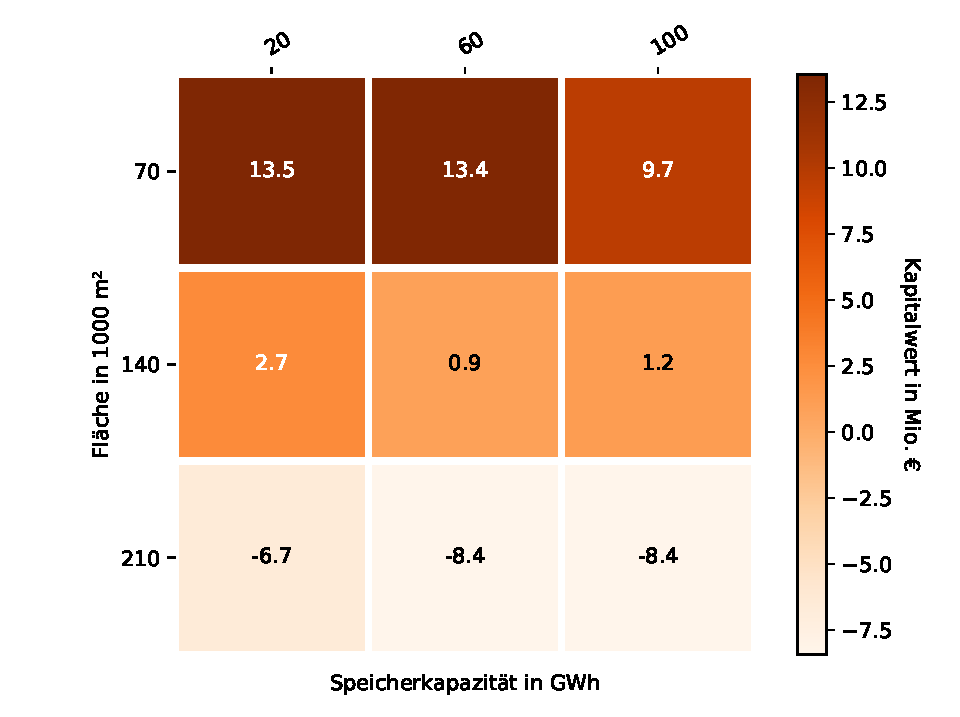
\includegraphics[width=1\textwidth]{Verbesserung/Solar2_Heatmap_relNPV-cropped.pdf}
			\subcaption{Solarthermie 2}
			\label{fig: Heatmaps Solarthermie b}
		\end{subfigure}
		\caption[Übersicht über die Kapitalwerte der Solarthermie Konzepte]{Übersicht über die Kapitalwerte des Solarthermie 1 (a) und Solarthermie 2-Konzepts (b) sowie aller betrachteten Szenarien in Form von Heatmaps. Dunkel dargestellte Flächen zeigen einen höheren Kapitalwert gegenüber den helleren Flächen an.}
		\label{fig: Heatmaps Solarthermie}
	\end{figure}

Wie die Abbildungen \ref{fig: Heatmaps Solarthermie} und \ref{figure: Heatmap Photovoltaik} zeigen, haben alle Konzepte gemeinsam, dass das wirtschaftlich attraktivste Szenario stets jenes mit der niedrigsten Kollektorfläche und geringsten Speicherkapazität ist. Bei dem Solarthermie~1 und Solarthermie~2 Konzept sorgen zunehmende Dimensionierungen der Anlagen dafür, dass der Kapitalwert negative Werte annimmt. Das bedeutet, dass der Betrieb dieser Szenarien, im Vergleich zum Referenzkonzept, unwirtschaftlich ist. Bei dem ST1-Konzept ist dies erst bei einer Kollektorfläche von 210.000~m² und einer Speicherkapazität von 60~GWh bzw. 100~GWh der Fall. Das ST2-Konzept weist ausschließlich negative Kapitalwerte bei einer Fläche von 210.000~m² auf. Demgegenüber zeigt sich, dass das \ac{PV}-Konzept stets positive Kapitalwerte annimmt (vgl. Abbildung \ref{figure: Heatmap Photovoltaik}).
	\begin{figure}[ht]
		\centering
		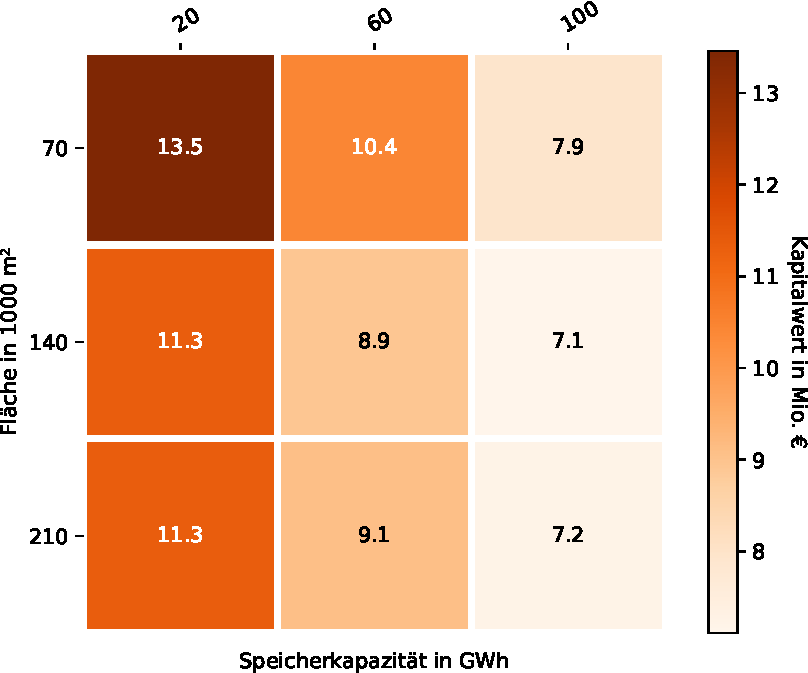
\includegraphics[width=0.8\textwidth]{PV_Heatmap_relNPV-cropped.pdf}
		\captionof{figure}[Darstellung aller Kapitalwerte innerhalb des Photovoltaik-Szenarios]{Darstellung einer Heatmap aller Kapitalwerte innerhalb des Photovoltaik-Szenarios. Dunkel dargestellte Fläche zeigen gegenüber helleren Flächen einen erhöhten Kapitalwert an.}
		\label{figure: Heatmap Photovoltaik}
	\end{figure}

Der höchste Kapitalwert mit 19,5~Mio.~\euro\ wird bei dem ST1-Konzept erreicht. Mit zunehmender Kollektorfläche auf 140.000~m² nimmt der Kapitalwert zunächst um 9,8~Mio.~\euro\ ab - bei einer Vergrößerung auf 210.000~m² um weitere 9,5~Mio.~\euro. Das zeigt, dass bei den gegebenen Umweltbedingungen eine zunehmende Kollektorfläche in dem betrachteten Bereich zu einer überproportionalen Abnahme des Kapitalwerts führt. Hieraus folgt, dass das Verhältnis aus gewonnenem Nutzen durch eine zunehmende Kollektorfläche und den zusätzlichen Kosten abnimmt. Außerdem kann an dieser Stelle zunächst davon ausgegangen werden, dass die optimale Kollektorfläche erst bei deutlich geringeren Werten erreicht wird. Bei einer Speicherkapazität von 60~GWh ist die Abnahme des Kapitalwerts ungefähr gleich der Abnahme bei 20~GWh. Erst bei der höchsten Kapazität von 100~GWh ist zu erkennen, dass die Abnahme des Kapitalwerts geringer wird. Bei einer Zunahme der Fläche auf 140.000~m² verringert sich der Kapitalwert an dieser Stelle nur um 7,5~Mio.~\euro. Daraus kann gefolgert werden, dass bei dieser Speicherkapazität die optimale Kollektorfläche größer ist und der Auslegungspunkt bei 70.000~m² somit dichter an einem lokalen Maximum liegt. Dies ist insofern plausibel, da davon ausgegangen werden kann, dass eine zunehmende Kollektorfläche einen größeren saisonalen Wärmespeicher erfordert. Analog dazu kann Abbildung \ref{fig: Heatmaps Solarthermie a}, aufgrund der relativ konstanten Abnahme des Kapitalwerts bei einer Steigerung der Kapazität von 60 auf 100~GWh, entnommen werden, dass die optimale Speichergröße unterhalb von 20~GWh liegt.

Abbildung \ref{fig: Heatmaps Solarthermie b} stellt die Kapitalwerte des ST2-Konzeptes dar. Wie bei dem ST1-Konzept ist der Kapitalwert bei einer Fläche von 70.000~m² und einer Speicherkapazität von 20~GWh am höchsten, liegt jedoch mit 13,5~Mio.~\euro\ etwas unter dem Ergebnis des ST1-Konzepts. Eine Zunahme der Kollektorfläche hat hier die selben Auswirkungen wie in ST1. Die Kapitalwerte fallen konstant um einen Wert von ca. 10~Mio.~\euro. Ebenso ist zu erkennen, dass die Abnahme bei einer Speicherkapazität von 60~GWh und 100~GWh zunächst geringfügig voneinander abweicht, bei einer Fläche von 140.000~m² und 210.000~m² jedoch gleich groß ist und zu identischen Kapitalwerten führt. In diesem Bereich scheinen sich der Nutzen und die zusätzlichen Kosten aufzuheben. Im Gegensatz zum ST1-Konzept ändert sich der Kapitalwert bei einer Zunahme der Speicherkapazität von 20 auf 60~GWh -~und konstant bleibender Fläche von 70.000~m²~- zunächst nur minimal, was darauf hindeutet, dass zwischen diesen Werten ein lokales Maximum zu finden ist.

Gegenüber den Solarthermie-Konzepten zeigen die \ac{PV}-Szenarien (Abbildung \ref{figure: Heatmap Photovoltaik}) ein etwas anderes Verhalten. Der höchste Kapitalwert liegt hier zwar ebenfalls bei der geringsten Fläche und Speicherkapazität, es wird jedoch bei zunehmender Kollektorfläche und Kapazität kein Kapitalwert negativ. Das heißt, dass alle Szenarien dem Referenzsystem aus ökonomischer Sicht vorzuziehen sind. Eine Zunahme der Modulfläche führt zunächst bei allen Speicherkapazitäten zu einer Abnahme des Kapitalwerts. Eine weitere Erhöhung der Fläche hat jedoch keinen weiteren Einfluss auf den Kapitalwert. Die gleichbleibenden Kapitalwerte bei 140.000 und 210.000~m² sprechen dafür, dass mit zunehmender Modulfläche ein anwachsender Anteil des \ac{PV}-Stroms am Spotmarkt vermarktet wird. Dies liegt daran, dass das \ac{PV}-System mit zunehmender Fläche entsprechend mehr am Spotmarkt agiert und somit eine zusätzliche Einnahmequelle vorliegt, die den zunehmenden Kosten zunächst entgegen wirkt. Der Punkt, an dem die zusätzlichen Investitions- und Betriebskosten den Nutzen durch größere Anlagendimensionierungen übersteigen, wird bei diesem Konzept deutlich später erreicht. 

	\begin{figure}[ht]
		\centering
		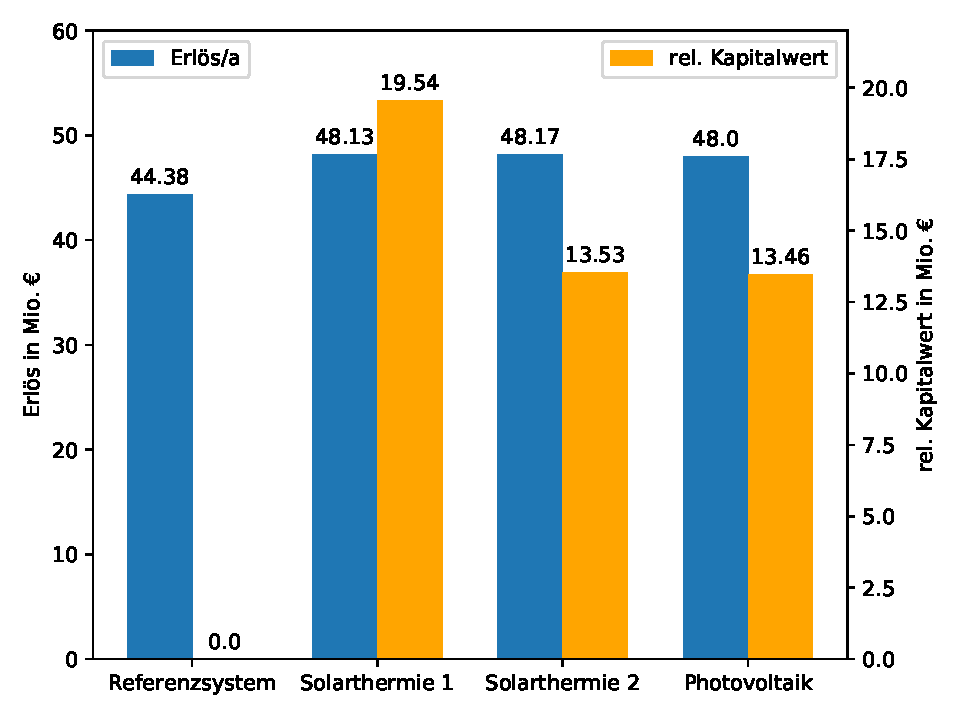
\includegraphics[width=0.8\textwidth]{Verbesserung/Erloes_K0_bester_Szenarien-cropped.pdf}
		\captionof{figure}[Gegenüberstellung der Erlöse und Kapitalwerte der wirtschaftlichsten Szenarien]{Darstellung der Erlöse und Kapitalwerte der verschiedenen Konzepte bei einer Kollektorfläche von 70.000~m² und einer Speicherkapazität von 20~GWh. Die Kapitalwerte der Alternativkonzepte werden auf das Referenzsystem bezogen, weshalb dieses mit einem Kapitalwert 0 angezeigt wird.}
		\label{figure: Erloes_K0_bester_Szenarien}
	\end{figure}

Abbildung \ref{figure: Erloes_K0_bester_Szenarien} stellt die, für eine genauere Untersuchung des Anlagenverhaltens ausgewählten Szenarien aller Konzepte vergleichend gegenüber. Es handelt sich hierbei stets um die Szenarien bei einer Kollektorfläche von 70.000~m² und einer Speicherkapazität von 20~GWh, da sich diese Auslegung als die wirtschaftlich attraktivste für alle Konzepte - unter den betrachteten Dimensionierungen - erwiesen hat. Es ist zu erkennen, dass im Betrachtungszeitraum alle Alternativkonzepte einen deutlich höheren Erlös gegenüber dem Referenzsystem erwirtschaftet haben. Trotzdem zeigt sich, dass der Kapitalwert des ST1-Konzepts erheblich größer ausfällt als beim ST2-, oder PV-Konzept. Dies ist über die zusätzlichen Investitionskosten der installierten Wärmepumpen zu erklären, die im PV-Konzept 12,5~Mio.~\euro\ und im ST2-Konzept 6,25~Mio.~\euro\ betragen. Darüber hinaus ist zu erkennen, dass die, durch eine zusätzlich installierte \ac{WP} und \ac{STTES} erhöhten Erlöse des Solarthermie~2 Konzepts, die Investitionskosten der Anlagen nicht kompensieren können.

Die folgenden Abschnitte werden das Anlagenverhalten innerhalb der ausgewählten Szenarien genauer betrachten. Außerdem wird für jedes Konzept eine Einflussanalyse durchgeführt, um zu identifizieren, welche Technologie welchen Einfluss auf das entsprechende Betriebsergebnis hat.

\subsubsection{Ergebnisse der Einsatzoptimierung Solarthermie 1}
Abbildung \ref{figure: Jahresdauerlinie_Solarthermie1} können die Jahresdauerlinien des Solarthermie 1 Konzeptes entnommen werden. Es zeigt sich, dass der Elektrodenheizkessel als Wärmeversorgungstechnologie fast komplett verdrängt worden ist - er wird über den betrachteten Zeitraum bloß 246~h betrieben. Die Betriebsstunden des \acl{SLK} bleiben hingegen fast identisch zum Referenzsystem - er wird mit 1870~h nur etwas weniger betrieben. Es ist jedoch zu erkennen, dass der \ac{SLK} deutlich länger im Nennbetriebspunkt betrieben wird. Ebenso hat sich der Betrieb des \ac{GuD} insofern verändert, dass die Betriebsstunden mit ca. 5.031~h im Vergleich zum Referenzsystem deutlich geringer ausfallen, die Anlage  jedoch erheblich länger unter Volllast betrieben wird. An dieser Stelle wird ausschließlich die Wärmebereitstellung des \ac{GuD} betrachtet.
	\begin{figure}[ht]
		\centering
		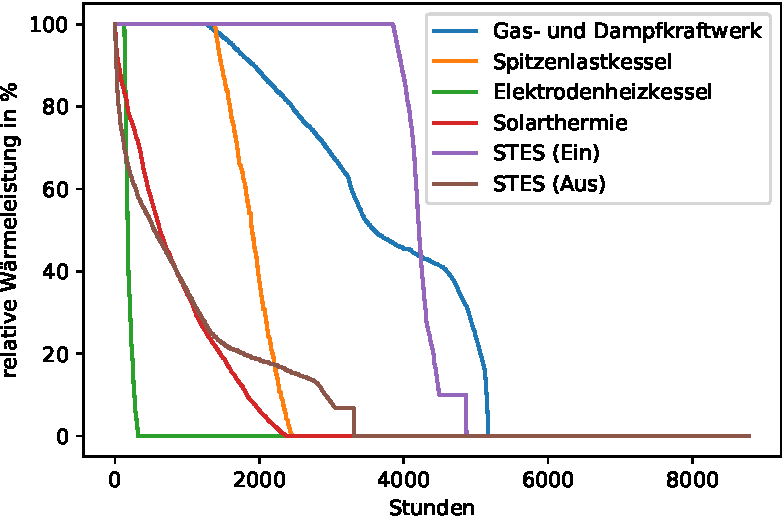
\includegraphics[width=0.8\textwidth]{Verbesserung/Jahresdauerlinie_Solarthermie1-cropped.pdf}
		\captionof{figure}[Jahresdauerlinien des Solarthermie 1-Konzepts]{Darstellung der Jahresdauerlinie aller verwendeten Technologien innerhalb des Solarthermie 1 Konzepts bei einer Kollektorfläche von 70.000~m² und einer Kapazität von 20~GWh}
		\label{figure: Jahresdauerlinie_Solarthermie1}
	\end{figure}
Die Jahresdauerlinie der Solarthermie-Anlage zeigt, dass nur wenige Stunden im Jahr eine volle Sonneneinstrahlung vorliegt. Erst ab einer Leistung von 60\% nehmen die Betriebsstunden der Anlage merklich zu. Insgesamt stellt die Solaranlage über das betrachtete Jahr 2.503~h Wärme bereit. 

Vergleicht man die Technologien hinsichtlich der insgesamt produzierten Wärme, liefert die \ac{GuD}-Anlage 84,77\% der Wärmeproduktion. Dies ist nur geringfügig unterhalb der anteiligen Produktion innerhalb des Referenzsystems. Ähnlich verhält es sich beim Betrieb des Spitzenlastkessels, der mit 7,32\% knapp 2,5 Prozentpunkte unterhalb des entsprechenden Werts im Referenzsystem liegt. Beim \ac{EHK} konnte bereits über die Betriebsstunden abgelesen werden, dass diese Technologie kaum einen Beitrag an der Wärmeproduktion leistet - nur 0,83\%. Die Solarthermie-Anlage schafft in diesem Konzept einen Anteil von 7,08\% an der gesamten Wärmeproduktion. Die Wärmegestehungskosten dieses Systems betragen 30,08~\euro/MWh und liegen damit 2,7~\euro/MWh unterhalb des Referenzsystem-Werts.

Bei dem Betrieb des \ac{STES} kann den Jahresdauerlinien entnommen werden, das er knapp 2500~h des Jahres mit dem maximal möglichen Wärmestrom geladen wird. Dem gegenüber ist der Speicher in dem betrachteten Jahr nie unter Volllast entladen worden. Die Fläche unterhalb der Kurven fürs Auf- und Entladen weichen deutlich voneinander ab, was an den unterschiedlich modellierten maximal möglichen Wärmeströmen liegt. Wie in Kapitel \ref{subsection: Solarthermie 1} beschrieben wurde, ist der Speicher so modelliert worden, dass er höchstens mit dem maximal möglichen Wärmestrom der Solaranlage geladen werden kann. Beim Entladen war der höchst mögliche Wärmestrom hingegen mit der maximalen Heizlast innerhalb des Jahres modelliert worden. Die Darstellung in Dauerlinien zeigt also, dass es besser gewesen wäre, die maximal mögliche Aufladung größer und die Entladung entsprechend geringer zu wählen.
	\begin{figure}
		\centering
		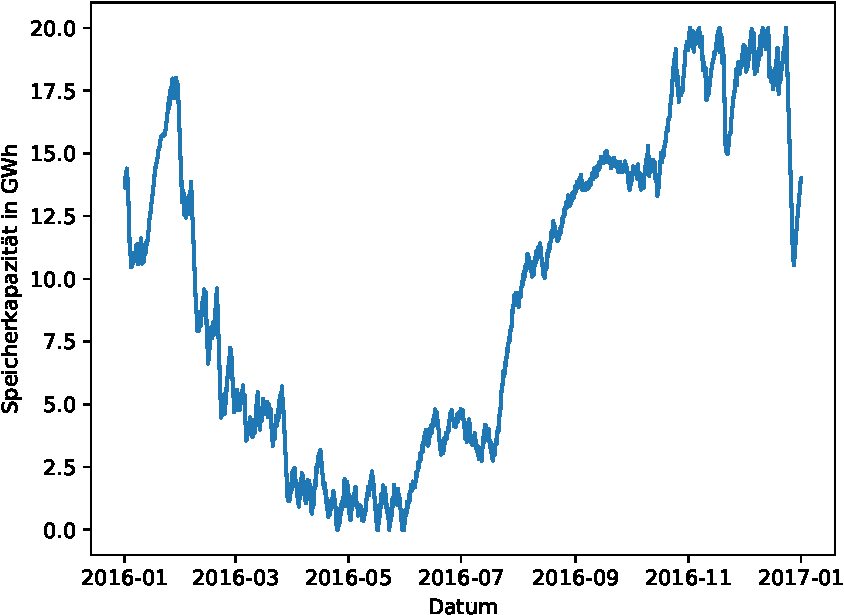
\includegraphics[width=0.8\textwidth]{Verbesserung/Speicherverhalten_Solarthermie1-cropped.pdf}
		\captionof{figure}[Ladezustand des saisonalen Wärmespeichers innerhalb des Solarthermie 1-Konzepts]{Illustration des Ladezustands des saisonalen Wärmespeichers innerhalb des Solarthermie 1-Konzepts über den betrachteten Zeitraum}
		\label{figure: Speicherkapazität_Solarthermie1}
	\end{figure}

Abbildung \ref{figure: Speicherkapazität_Solarthermie1} zeigt zu jedem Zeitpunkt des betrachteten Jahres den Ladezustand des Wärmespeichers. Nachdem zunächst ca. 2~GWh aus dem Speicher entnommen werden, wird er im Februar bis auf ca. 17,5~GWh geladen. Daran anschließend wird der Speicher bis in den Mai überwiegend entladen. Von Anfang Juni bis Ende Juli bildet sich eine kleine Erhöhung aus, in der der Speicher wieder auf knapp 5~GWh geladen wird. Von August bis November wird der Speicher primär aufgeladen. Im Winter wird er mehrmals entladen - wird aber in kurzer Zeit wieder auf die maximale Kapazität aufgeladen. Dieses Verhalten ist durch tendenziell erhöhte Strompreise und den damit einhergehenden Betrieb der \ac{GuD}-Anlage zu erklären. Welchen Einfluss die Solarthermie auf den Verlauf der Speicherkapazität hat wird in der an diesen Abschnitt angrenzenden Einflussanalyse untersucht.
	\begin{figure}
		\centering
		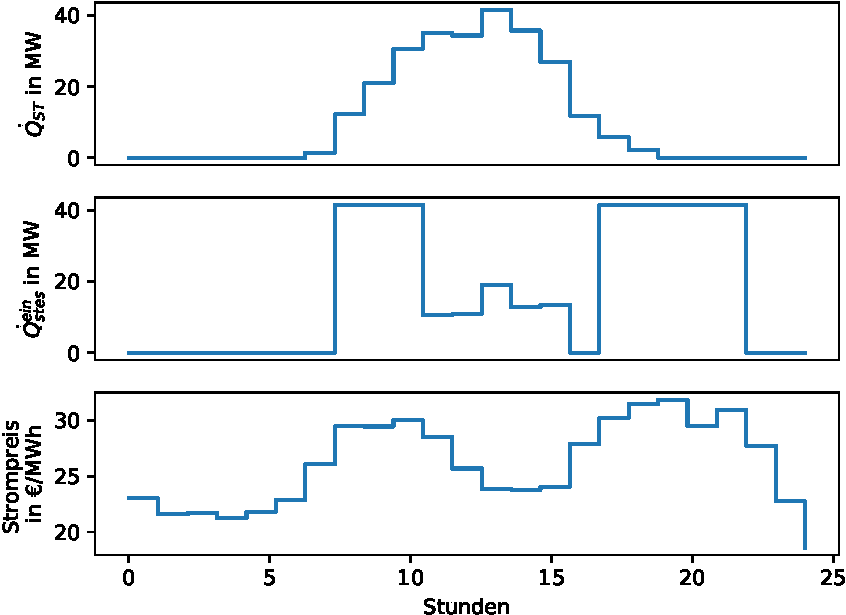
\includegraphics[width=0.8\textwidth]{Verbesserung/Solarthermie_1_Verhalten-cropped.pdf}
		\captionof{figure}[Darstellung der solaren Wärme über Speicherbeladung und Strompreis für das ST1-Konzept]{Darstellung der solaren Wärme $\dot{Q}_{ST}$ über dem Speicher zugeführten Wärmestrom $\dot{Q}_{stes}^{ein}$ sowie den Strompreisen für den 11.06.2016 - den Tag mit der höchsten Sonneneinstrahlung im Betrachtungszeitraum}
		\label{figure: Verhalten_Solarthermie1}
	\end{figure}
	
Zunächst soll jedoch veranschaulicht werden nach welchen Prinzipien der Speicher beladen wird. Zu diesem Zweck wird in Abbildung \ref{figure: Verhalten_Solarthermie1} der Solarthermie-Ertrag über dem Wärmestrom in den \ac{STES} und jeweiligen Strompreisen am Spotmarkt dargestellt. Es ist sofort zu erkennen, dass der Speicher - trotz des erheblichen Wärmestroms aus der Solarthermie - primär durch die \ac{GuD}-Anlage aufgeladen wird. Dies kann daraus abgeleitet werden, dass die Aufladung des Speichers mit dem Strompreis korreliert. Ein erhöhter Strompreis am Spotmarkt führt dazu, dass das \ac{GuD} verstärkt betrieben wird. Gleichzeitig kann Abbildung \ref{figure: Verhalten_Solarthermie1} entnommen werden, dass zumindest ein Teil der durch die Solarthermie bereitgestellten Wärme genutzt wird, um den Speicher zu laden. Dies ist zwischen Stunde 11 und Stunde 16 der Fall.

\subsubsection*{Einflussanalyse des ST1-Konzepts}
Abbildung \ref{figure: Erloes_K0_bester_Szenarien} hat bereits gezeigt, dass das Solarthermie 1 Konzept - die Einbringung einer Solarthermie-Anlage und eines saisonalen Wärmespeichers - einen ökonomischen Vorteil gegenüber dem Referenzsystem darstellt. An dieser Stelle wird kurz untersucht, welchen Beitrag die einzelnen Technologien zu diesem Ergebnis geleistet haben.

Um den Einfluss der Solarthermie und des \ac{STES} zu untersuchen sind diese Technologien einzeln dem Referenzsystem hinzugefügt worden. Zunächst soll der Einfluss des \ac{STES} untersucht werden. Zu diesem Zweck ist der Solarthermie-Ertrag innerhalb des ST1-Konzepts auf 0 gesetzt worden. Es zeigt sich nach Abbildung \ref{fig: Jahresdauerlinie_Einfluss_ST1}, dass das Referenzsystem einzig durch den Einsatz eines Wärmespeichers deutlich effizienter betrieben werden kann. Der Speicher sorgt für eine Entkopplung der Wärmeproduktion sowie des Bedarfs und führt somit dazu, dass das \ac{GuD} verstärkt bei Nennlast Wärme bereitstellt. 

Ein Vergleich der Jahresdauerlinien ohne Solarthermie zeigt darüber hinaus, dass sich das Betriebsverhalten der Anlagen kaum von dem System mit Solarthermie unterscheidet. Der \ac{EHK} ist genauso aus der Wärmeproduktion verdrängt worden, was zeigt, dass die Verdrängung einzig an der Verwendung eines Wärmespeichers liegt. Demgegenüber zeigt die übers Jahr aufgetragene relative Speicherkapazität in Abbildung \ref{fig: Speicherkapazität_Einfluss_ST1}, in der die Differenz zwischen dem Ladezustand des Systems mit und ohne Solarthermie abgebildet wird, einen deutlichen Unterschied des Ladeverhaltens. Es ist zu erkennen, dass der Ladezustand des Speichers zwischen August und Ende Oktober ohne Wärme aus der Solarthermie um bis zu 6~GWh niedriger ist. Dies zeigt, dass Solarthermie durchaus saisonal gespeichert wird und stützt somit das in Abbildung \ref{figure: Verhalten_Solarthermie1} dargestellte Verhalten, dass die Wärme aus der Solarthermie anteilig zur Ladung des Speichers genutzt wird. Ein kleinerer Ausschlag ist im März erkennbar. Zu dieser Zeit werden die ersten nennenswerten Erträge über die Solarthermie bereitgestellt. Zwischen diesen Zeiträumen unterscheidet sich der Ladezustand um maximal 1~GWh, was dafür spricht, dass die Solarthermie zu dieser Zeit mit einer niedrigen Wärmelast bevorzugt direkt zur Wärmebereitstellung genutzt wird.
	\begin{figure}
		\begin{subfigure}[b]{0.48\textwidth}
			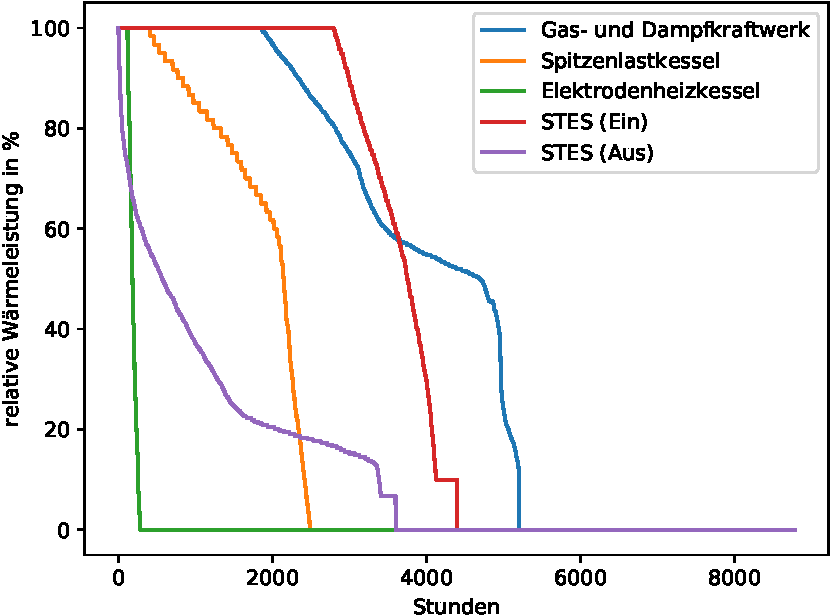
\includegraphics[width=1\textwidth]{Verbesserung/ST1_Jahresdauerlinie_Einfluss_STES-cropped.pdf}
			\subcaption{Jahresdauerlinien}
			\label{fig: Jahresdauerlinie_Einfluss_ST1}
		\end{subfigure}
		\hfill
		\begin{subfigure}[b]{0.48\textwidth}
			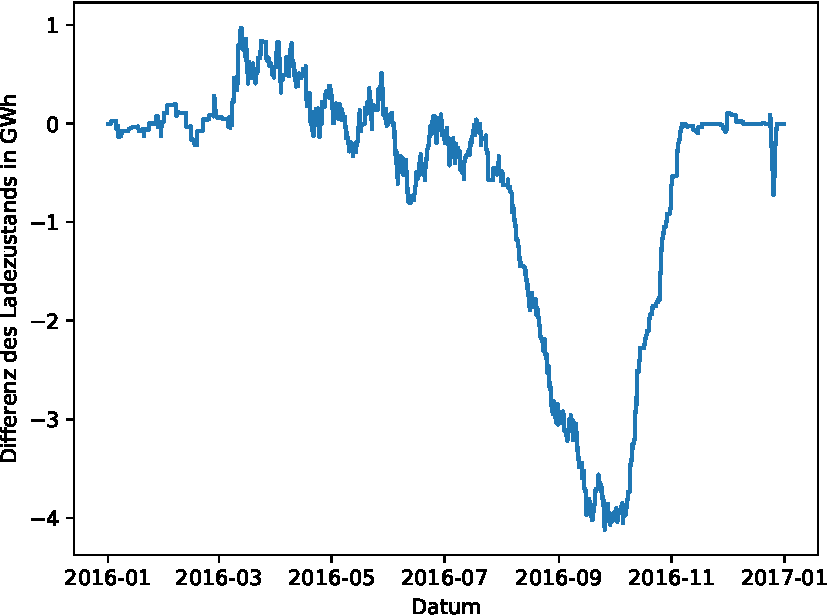
\includegraphics[width=1\textwidth]{Verbesserung/ST1_relSpeicherkap_Einfluss_STES-cropped.pdf}
			\subcaption{relative Speicherkapazität}
			\label{fig: Speicherkapazität_Einfluss_ST1}
		\end{subfigure}
		\caption[Verhalten der Anlagen des ST1-Konzepts ohne den Ertrag aus der Solarthermie-Anlage]{Verhalten der Anlagen des ST1-Konzepts ohne den Ertrag aus der Solarthermie-Anlage. In (a) werden die Jahresdauerlinien dargestellt, während in (b) die Differenz beim Ladezustand zwischen dem ST1-Konzept mit und ohne Solarthermie dargestellt wird. Ein negative Ausschlag bedeutet, dass der Ladezustand des Speichers mit Solarthermie zu diesem Zeitpunkt höher ist.}
		\label{fig: Einfluss}
	\end{figure}


Aus rein ökonomischer Sicht zeigt sich, dass das Hinzufügen eines Wärmespeichers - zur Entkopplung der Wärmeproduktion und des Bedarfs - attraktiver ist, als die Kombination aus Solarthermie und Speicher. Der Kapitalwert des Referenzsystems steigt allein durch den Wärmespeicher mit einer Kapazität von 20~GWh um 33,16~Mio.~\euro, was ungefähr 170\% der Kombination aus Solarthermie und Speicher entspricht. Gleichzeitig sinkt der Kapitalwert des Referenzsystems um 17,71~Mio.~\euro, wenn ausschließlich eine Solaranlage mit 70.000~m² hinzugefügt wird. Der fehlende Speicher sorgt dafür, dass es nicht möglich ist 100\% des Solar-Ertrags zu verwenden. Tatsächlich werden ohne einen Speicher nur ca. 1/4 der solarthermischen Wärme genutzt. Dies sorgt für den niedrigen Kapitalwert. 

Die Einflussanalyse des Solarthermie 1-Konzepts hat gezeigt, dass bei den zugrunde gelegten regulatorischen Rahmenbedingungen und Brennstoffkosten aus rein ökonomischer Sicht die einfache Ergänzung des Referenzsystems um einen Wärmespeicher die attraktivste Maßnahme darstellt. Dies wird in Tabelle \ref{tabelle: Übersicht Einflussanalyse ST1} veranschaulicht. Es ist klar zu erkennen, dass das Ergebnis des ST1-Konzepts hauptsächlich aufgrund des verwendeten Speichers gut ausfällt. Die Verwendung der Solarthermie erhöht den Erlös nur um 400.000~\euro, senkt den Kapitalwert durch die hohen Investitionskosten jedoch erheblich. 
	\begin{center}
		\captionof{table}{Übersicht über die Ergebnisse der Einflussanalyse des Solarthermie 1-Konzepts} 
		\label{tabelle: Übersicht Einflussanalyse ST1}
		\begin{tabular}{lcccc}
			\hline 
			 &  & Erlös M\euro/a & Kapitalwert M\euro & \ac{LCOH} \euro/MWh\tabularnewline
			 
			\hline 
			Solarthermie 1 (normal)  &  & 48,13 & 19,5 & 30,08 \tabularnewline
			nur mit \ac{STES}		 &  & 47,68 & 33,16 & 28,26 \tabularnewline
			nur mit Solarthermie 	 &  & 44,48 & -17,71 & 35,08 \tabularnewline		
			\hline
		\end{tabular}
	\end{center}

\subsubsection{Ergebnisse der Einsatzoptimierung Solarthermie 2}
Das Solarthermie 2-Konzept stellt mit einer zusätzlichen Wärmepumpe und einem Kurzzeitspeicher (\acs{STTES}) ein Konzept dar, bei dem die Solarthermie mit anderen Technologien zur Wärmebereitstellung kombiniert wird. Die \ac{WP} sollte den Anteil an \ac{P2H} in dem Wärmeversorgungssystem erhöhen und somit ein Wärmesystem mit erhöhtem \ac{P2H}-Anteil abbilden. Wie bereits im vorangegangen Abschnitt zum ST1-Konzept, soll an dieser Stelle das Betriebsverhalten der Anlagen - als Ergebnis der Einsatzoptimierung - genauer betrachtet werden. Daran anschließend wird eine Einflussanalyse durchgeführt, die den Einfluss der neu hinzugekommenen Technologien auf das Betriebsergebnis untersuchen wird. 

Die Jahresdauerlinien des Solarthermie 2-Konzepts werden in \ref{figure: Jahresdauerlinie_Solarthermie2} dargestellt. Aufgrund der Tatsache, dass die Solarthermie als fixe Eingangsgröße in das Optimierungsmodell abgebildet worden ist, unterscheidet sich der Betrieb der Solaranlage nicht von dem aus ST1. Wie beim ST1-Konzept ist der \ac{EHK} als Wärmeversorgungstechnologie hier ebenfalls fast komplett verdrängt worden - interessanterweise bleibt der Anteil an der Wärmeproduktion, trotz der zusätzlichen \acl{WP}, nahezu unverändert. Gleiches gilt für den Betrieb des \ac{SLK}, der in diesem Konzept nur 35~h weniger als beim ST1-Konzept betrieben wird. Ein entgegengesetzter Effekt ist beim Betrieb des \ac{GuD} zu beobachten, welches mit 4.684 Betriebsstunden zwar knapp 350~h weniger im Betrachtungszeitraum betrieben wurde - jedoch 700~h länger unter Volllast Wärme bereitgestellt hat. Dies ist vor allem durch die Verwendung des Kurzzeitspeichers zu erklären, der im Gegensatz zum modellierten \ac{STES} auf stündlicher Basis ge- und entladen werden kann. Zur Wärmepumpe ist zu sagen, dass sie überwiegend zwischen 60\% und 70\% gearbeitet hat. Dies liegt unter anderem daran, dass die Leistungszahl von den Umweltbedingungen und der Vorlauftemperatur des Netzes abhängt, und diese über weite Teile des Jahres keinen optimalen Betrieb erlauben.
	\begin{figure}[ht]
		\centering
		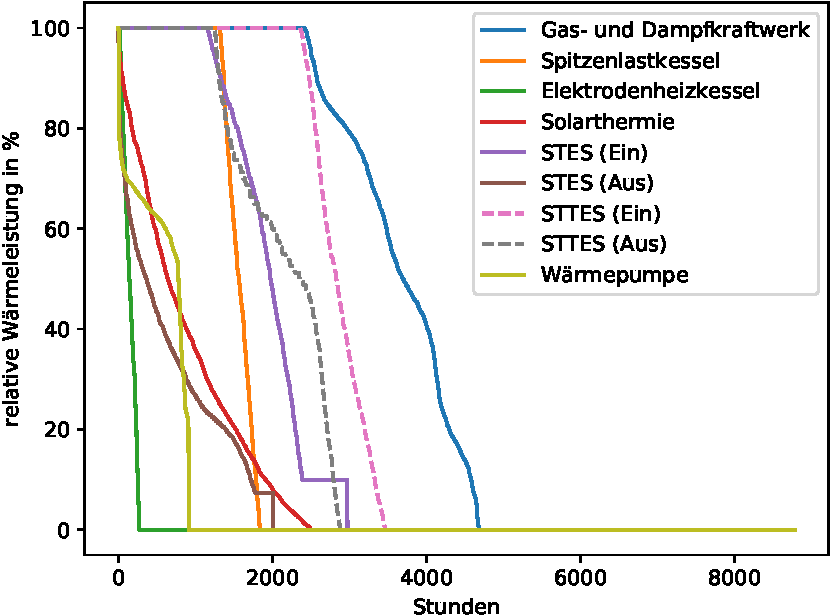
\includegraphics[width=0.8\textwidth]{Verbesserung/Jahresdauerlinie_Solarthermie2-cropped.pdf}
		\captionof{figure}[Jahresdauerlinie Solarthermie 2]{Abbildung der Jahresdauerlinien des Solarthermie 2-Konzepts. Dargestellt wird die relative Wärmeleistung der verwendeten Technologien über den Betriebsstunden bei einer Kollektorfläche von 70.000~m² und einer Speicherkapazität von 20~GWh}
		\label{figure: Jahresdauerlinie_Solarthermie2}
	\end{figure}

Anhand der Jahresdauerlinie ist zu erkennen, dass der \ac{STES} deutlich weniger genutzt wird als im ST1-Szenario. Der Verlauf der Be- und Entladung hat sich jedoch prinzipiell nicht verändert. Zum Großteil wird der Speicher noch immer unter Volllast aufgeladen, während das Entladen hauptsächlich in Teillast erfolgt. Die Gründe sind dieselben wie bereits beim ST1-Konzept. Der Kurzzeitspeicher wird zum größten Teil unter Volllast aufgeladen. Die Entladung findet zu ungefähr der Hälfte unter Volllast statt. Der Unterschied zwischen beiden Kurven liegt beim Kurzzeitspeicher einzig an dem Wirkungsgrad von 75\%. 

Das Speicherverhalten hat sich im Vergleich zum ST1-Konzept nur geringfügig verändert. Dominiert wird das Verhalten immer noch von den Strompreisen - hohe Strompreise führen zu einem wirtschaftlichen Betrieb der \ac{GuD}-Anlage, welche dann zum Laden des Speichers genutzt wird. Um das Anlagenverhalten zu veranschaulichen ist in Abbildung \ref{figure: Verhalten_Solarthermie2} die solarthermisch gewonnene Wärme für den 09. und 10.05.2016 über der Speicherbeladung $\dot{Q}^{ein}$, dem Wärmestrom der Wärmepumpe $\dot{Q}_{WP}$ und den Strompreisen aufgetragen. Es ist zu erkennen, dass der saisonale Speicher und der Kurzzeitspeicher ähnlich geladen werden. Ein erhöhter Strompreis am Morgen und Abend führt bei beiden Speichern zu einer Beladung mit dem maximal möglichen Wärmestrom. Die Wärmepumpe wird in dem Beispiel nachts bei fehlender Solarthermie genutzt, um Wärme bereitzustellen - diese wird ausschließlich ins Netz eingespeist. Die solarthermische Wärme wird wie in ST1 anteilig zur Speicherung genutzt. An den dargestellten Tagen wird jedoch vorzugsweise der Kurzzeitspeicher genutzt. 
	\begin{figure}
		\centering
		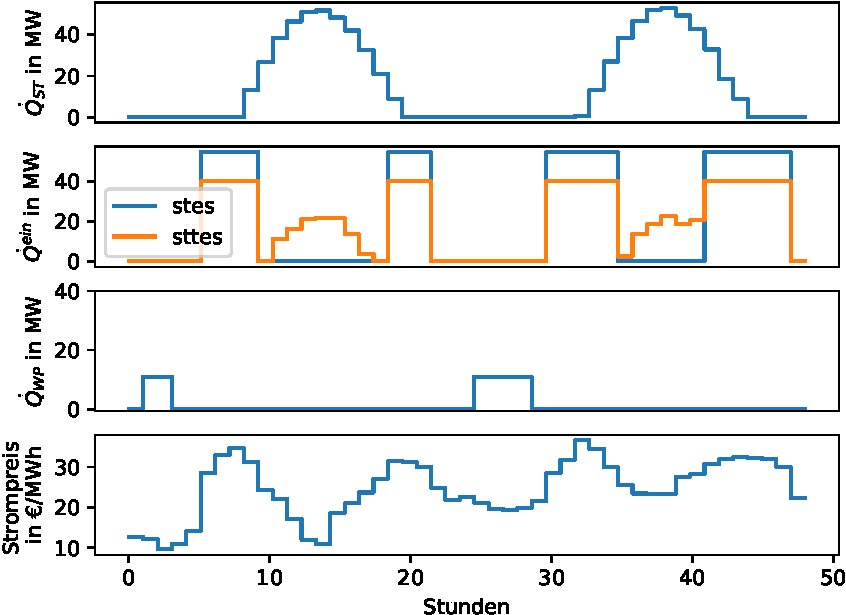
\includegraphics[width=0.8\textwidth]{Verbesserung/Solarthermie_2_Verhalten_09_05-cropped.pdf}
		\captionof{figure}[Illustration der solaren Wärme über Speicherbeladung und Strompreis für das ST2-Konzept]{Illustration des Solarthermie-Ertrags $\dot{Q}_\text{ST}$, der Speicherbeladung $\dot{Q}^{ein}$ des \ac{STES} und \ac{STTES} über der Wärmeabgabe durch die Wärmepumpe $\dot{Q}_{WP}$ und den Strompreisen für den 09/10.05.2016}
		\label{figure: Verhalten_Solarthermie2}
	\end{figure}

Insgesamt hat sich die Wärmeproduktion innerhalb des ST2-Szenarios kaum verändert. Der Anteil des \ac{GuD} ist weiter auf 82,39\% gesunken - stellt jedoch weiterhin die dominierende Technologie dar. Die Wärmeproduktion des \ac{SLK} hat sich auf 7,20\%  und die des \ac{EHK} auf 0,69\% reduziert. Die Wärmeproduktion der \ac{WP} beträgt anteilig an der gesamten Produktion 2,75\% und ist für die reduzierten Anteile der anderen Technologien verantwortlich. Der Solarthermie-Anteil bleibt im Wesentlichen unverändert.

\subsubsection*{Einflussanalyse des ST2-Konzepts}
Bereits für das ST1-Szenario ist der Einfluss der Solarthermie und des \ac{STES} auf das Ergebnis der Optimierung untersucht worden. Dieser Abschnitt befasst sich daher ausschließlich mit der Wärmepumpe sowie dem Kurzzeitspeicher und deren Auswirkungen auf das ST2-Konzept.

Zunächst wird der Einfluss der Wärmepumpe untersucht indem diese aus der Optimierung entfernt wird. Es zeigt sich, dass durch die zusätzliche \ac{WP} das Betriebsergebnis des ST1-Konzept quasi nicht verbessert wird. Der Erlös mit einer zusätzlich installierten Wärmepumpe hat sich um 0,04~Mio.~\euro\ erhöht. Eine Umverteilung der Wärmeproduktion durch den Einsatz der Wärmepumpe hat also nur einen geringen Einfluss auf das Betriebsergebnis der Optimierung. Durch die zusätzlichen Investitionskosten hat sich der Kapitalwert des Konzepts jedoch auf 13,5~Mio.~\euro\ reduziert. 

Ein anderer Effekt ist zu beobachten, wenn ausschließlich der Kurzzeitspeicher als Ergänzung zum ST1-Konzept betrachtet wird. In diesem Fall erhöht sich der Kapitalwert auf 18,63~Mio.~\euro\ und liegt damit nur knapp unterhalb dem Kapitalwert des ST1-Konzepts. Offenbar hat der zusätzliche Speicher einen positiven Einfluss auf das Betriebsergebnis. Liegt diese Verbesserung jedoch an dem zusätzlichen Speicher, der stündlich ge- und entladen werden kann und somit einen parallelen Betrieb zum \ac{STES} ermöglicht, oder ruht die Verbesserung in der Tatsache, dass insgesamt ein höherer Wärmestrom gespeichert werden kann. Um diese Frage zu beantworten ist der maximal mögliche Wärmestrom zur Beladung des \ac{STES} verdoppelt (dies entspricht ungefähr der Summe des \ac{STES} und \ac{STTES}) und eine Betriebsoptimierung ohne einen Kurzzeitspeicher durchgeführt worden. Es zeigt sich, dass allein durch einen größeren Wärmestrom, mit dem der \ac{STES} beladen wird, ein deutlich besseres Betriebsergebnis erreicht wird. Darüber hinaus führt dies zu einer, mit 2631~h unter Volllast, effizienteren Nutzung des \ac{GuD}. Der Kapitalwert steigt auf 21,95~Mio.~\euro\ und liegt -~aufgrund der fehlenden Investitionskosten für den zusätzlichen Speicher~- oberhalb des Kapitalwerts des \ac{STTES}-Systems. Dieses Ergebnis zeigt, welchen Einfluss die Beladung des Speichers auf die Optimierung hat und dass der angenommene, maximale Wärmestrom im Prinzip zu niedrig angesetzt worden ist.

Abgesehen von dem Betriebsergebnis hat der zusätzliche Wärmespeicher jedoch einen erheblichen Einfluss auf die Art und Weise, wie der \ac{STES} betrieben wird. Abbildung \ref{fig: Einfluss_Speicher_Solar_2} stellt den Ladezustand des saisonalen Speichers gegenüber. Die Grafik \ref{fig: Speicherkapazität_ST2} illustriert hier das Speicherverhalten des \ac{STES} bei Verwendung eines Kurzzeitspeichers. Demgegenüber stellt Grafik \ref{fig: Speicherkapazität_Einfluss_ST2} den Ladezustand ohne die Verwendung eines Kurzzeitspeichers dar. Es ist zu erkennen, dass ein zusätzlicher Speicher den Betrieb des \ac{STES} glättet. Die Verwendung eines zusätzlichen Speichers hat also einen erheblichen Einfluss auf die Betriebsweise des \ac{STES}.
	\begin{figure}[ht]
		\begin{subfigure}[b]{0.48\textwidth}
			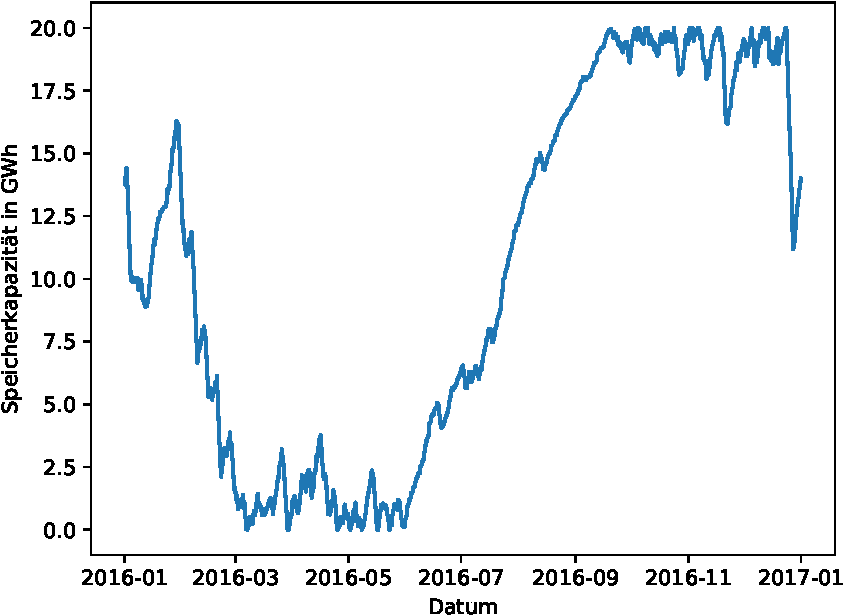
\includegraphics[width=1\textwidth]{Verbesserung/Speicherverhalten_Solarthermie2-cropped.pdf}
			\subcaption{mit \ac{STTES}}
			\label{fig: Speicherkapazität_ST2}
		\end{subfigure}
		\hfill
		\begin{subfigure}[b]{0.48\textwidth}
			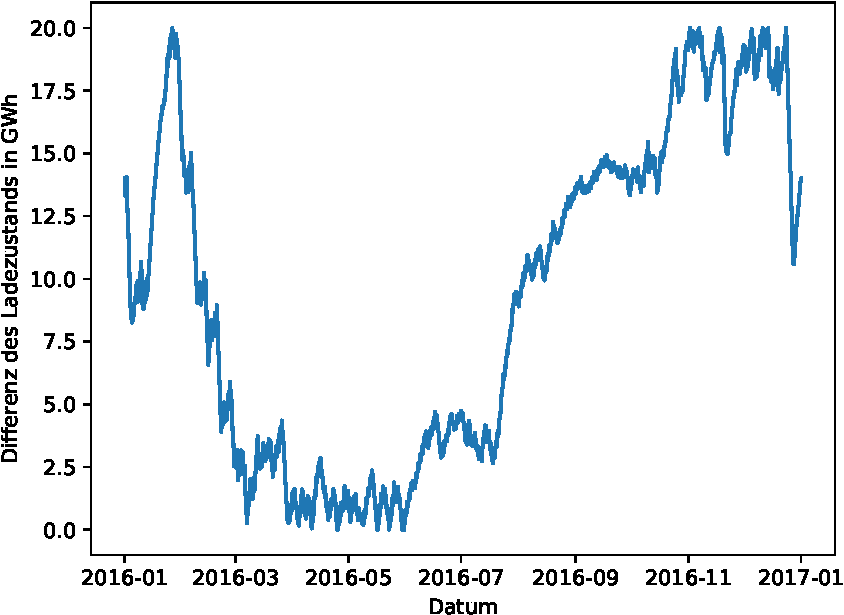
\includegraphics[width=1\textwidth]{Verbesserung/Speicherverhalten_Solarthermie2_woSTTES-cropped.pdf}
			\subcaption{ohne \ac{STTES}}
			\label{fig: Speicherkapazität_Einfluss_ST2}
		\end{subfigure}
		\caption[Vergleich des saisonalen Speicherverhaltens mit und ohne Kurzzeitspeicher]{Gegenüberstellung des saisonalen Speicherverhaltens mit und ohne Kurzzeitspeicher. In Teil (a) wird der Ladezustand des Speichers mit Kurzzeitspeicher - in Teil (b) ohne dargestellt.}
		\label{fig: Einfluss_Speicher_Solar_2}
	\end{figure}

Tabelle \ref{tabelle: Übersicht Einflussanalyse ST2} fasst die ökonomischen Ergebnisse der Einflussanalyse kurz zusammen. Die Tatsache, dass der Erlös der Optimierung nur mit \acl{STTES} höher ist, als der Erlös des normalen ST2-Konzepts ist über die Genauigkeit des Solvers (1\%) zu erklären.
\newpage
	\begin{center}
		\captionof{table}{Übersicht über die Ergebnisse der Einflussanalyse des Solarthermie 2-Konzepts} 
		\label{tabelle: Übersicht Einflussanalyse ST2}
		\begin{tabular}{lcccc}
			\hline 
			&  & Erlös M\euro/a & Kapitalwert M\euro & \ac{LCOH} \euro/MWh\tabularnewline
			
			\hline 
			Solarthermie 2 (normal)  &  & 48,17 & 13,53 & 30,88 \tabularnewline
			nur mit \ac{WP}			 &  & 48,00 & 11,83 & 31,11\tabularnewline
			nur mit \ac{STTES} 		 &  & 48,08 & 18,63 & 30,19\tabularnewline
			ST1 mit doppelter Beladung 		 & & 48,31 & 21,95 & 29,76\tabularnewline		
			\hline
		\end{tabular}
	\end{center}

\subsubsection{Ergebnisse der Einsatzoptimierung Photovoltaik}
Das \acl{PV}-Konzept stellt eine Alternative zur herkömmlichen Solarthermie dar und ist, als Konzept indirekter solarthermischer Wärme, mit dem ST1-Konzept verglichen worden. Die in Abbildung \ref{figure: Jahresdauerlinie_Photovoltaik} dargestellten Anlagen zeigen ein ähnliches Verhalten, wie es bereits im ST1 und ST2-Konzept beobachtet werden konnte. Der \ac{EHK} ist als Technologie quasi komplett aus der Wärmeversorgung verdrängt worden. Der \ac{EHK} wird innerhalb des \ac{PV}-Konzepts nur 480~h betrieben - der Anteil an der Wärmeproduktion hat sich auf 0,42\% reduziert. Analog verhält es sich beim Betrieb des Spitzenlastkessels, der, wie in den vorangegangenen Konzepten, mit 2123~h und einer anteiligen Wärmeproduktion von 8,02\% auch in diesem Konzept einen erheblichen Beitrag zur Wärmeversorgung leistet. Im Vergleich zu ST1 ist erkennbar, dass das \ac{GuD} länger unter Volllast und somit effizienter betrieben wird. Die Wärmepumpen sind in der Jahresdauerlinie zu einer einzigen Komponente zusammengefasst worden. Es werden zwei Wärmepumpen der selben Auslegung (ST2) verwendet, um garantieren zu können, dass 100\% des \ac{PV}-Stroms zur Wärmebereitstellung genutzt werden können.   Mit 1437 Betriebsstunden sind die Wärmepumpen in diesem Konzept knapp 500~h länger als in ST2 betrieben worden. Gegenüber dem ST2-Konzept, in dem die Wärmepumpe quasi nur zwischen 60 und 70\% ihrer maximalen Leistung betrieben worden ist, werden die Wärmepumpen in diesem über ein breiteres Spektrum betrieben. Insgesamt liegt die anteilige Wärmeproduktion der \ac{WP} bei 5,5\%. 
	\begin{figure}[ht]
		\centering
		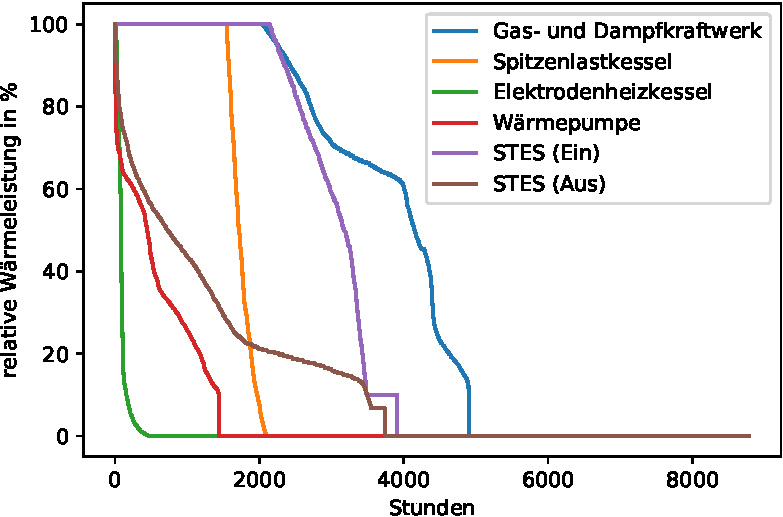
\includegraphics[width=0.8\textwidth]{Jahresdauerlinie_Photovoltaik-cropped.pdf}
		\captionof{figure}[Jahresdauerlinien Photovoltaik]{Illustration des Anlagenbetriebs innerhalb des Photovoltaik-Konzepts als Jahresdauerlinien. Es ist die relative Wärmeleistung der Anlage über den Betriebsstunden bei einer Modulfläche von 70.000~m² und einer Speicherkapazität von 20~GWh dargestellt.}
		\label{figure: Jahresdauerlinie_Photovoltaik}
	\end{figure}

Es stellt sich nunmehr die Frage, welchen Anteil der durch die \ac{PV}-Anlage bereitgestellte Strom zum Betrieb der Wärmepumpe - wie es in diesem Konzept vorgesehen ist - genutzt wurde. Zu diesem Zweck ist der \ac{PV}-Ertrag mit der elektrischen Leistung der Wärmepumpen verglichen worden. Sofern der Bedarf der \ac{WP} den Ertrag der \ac{PV}-Anlage überschreitet, ist angenommen worden, dass 100\% des \ac{PV}-Stroms zum Betrieb der \ac{WP} genutzt wurde. Übersteigt die elektrische Leistung der \ac{PV}-Anlage den Bedarf der \ac{WP}, ist angenommen worden, dass diese komplett durch \ac{PV} betrieben wird. 

Es zeigt sich, dass 33,53\% des \ac{PV}-Stroms zur Wärmebereitstellung durch die Wärmepumpen genutzt wird - 66,47\% werden am Spotmarkt vermarktet. Über die jeweiligen Leistungszahlen kann die entsprechende Wärmeproduktion - allein durch \ac{PV} - auf 9348,26~MWh berechnet werden. Dies entspricht 1,43\% an der gesamten Wärmeproduktion (ca. 1/3 im Vergleich zur Solarthermie) und nimmt somit eine eher untergeordnete Rolle bei der Wärmeversorgung ein. Abbildung \ref{figure: Verhalten_PV} soll das Verhalten der Wärmepumpe weiter veranschaulichen. Dargestellt wird der Ertrag der \ac{PV}-Module über dem von den Wärmepumpen in Summe abgegebenen Wärmestrom $\dot{Q}_{\textit{WP}}$ und dem Strompreis für den 11.06. und 12.06.2016. Es ist deutlich zu erkennen, dass auch mit hohem \ac{PV}-Ertrag die Wärmepumpe ausschließlich bei niedrigen Strompreisen betrieben wird - andernfalls ist es wirtschaftlicher, den Strom am Spotmarkt zu vermarkten. Darüber hinaus ist zu erkennen, dass bei entsprechend hohem \ac{PV} Dargebot die \ac{WP} ausschließlich über die \ac{PV}-Anlage betrieben wird. Dies ist an 248 Stunden des Jahres der Fall.
	\begin{figure}[ht]
		\centering
		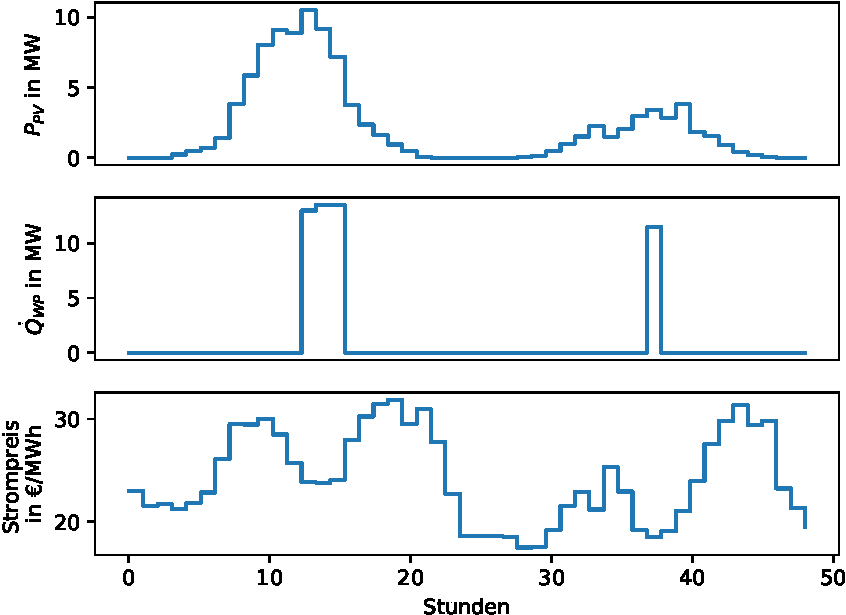
\includegraphics[width=0.8\textwidth]{Photovoltaik_Verhalten_11_06-cropped.pdf}
		\captionof{figure}[Illustration des PV- und Wärmepumpen-Ertrags über dem Strompreis]{Illustration des PV-Ertrags $P_{PV}$, dem von den Wärmepumpen in Summe abgegebenen Wärmestrom $\dot{Q}_{WP}$ über dem Strompreis für den 11.06. und 12.06.2016}
		\label{figure: Verhalten_PV}
	\end{figure}

Auf eine Darstellung des saisonalen Wärmespeichers wird an dieser Stelle verzichtet. Der Ladezustand des Speichers hat einen ähnlichen Verlauf wie der Speicher im ST1-Konzept. Zwischen August und Oktober wird der Speicher innerhalb dieses Konzepts auf einen höheren Stand geladen - ansonsten gleichen sich die Verläufe jedoch stark. Eine Abbildung des über das Jahr aufgetragenen Ladezustands kann dem Anhang (\ref{Anhang: Ladezustand}) entnommen werden.

\subsubsection*{Einflussanalyse des Photovoltaik-Konzepts}
Bereits in der Einflussanalyse zum ST1-Konzept ist der Einfluss des saisonalen Speichers untersucht worden. Es hat sich gezeigt, dass der saisonale Speicher den Einsatz der Anlagen, durch die Entkopplung von Erzeugung und Bedarf, erheblich verbessert. Für die Wärmepumpe in der Einflussanalyse zum ST2-Konzept konnte dargelegt werden, dass diese an sich den Betrieb nur minimal verbessert - in diesem Fall bestand jedoch nicht die Möglichkeit die Wärmepumpe regenerativ über den Strom einer \ac{PV}-Anlage zu betreiben. Aus diesem Grund wird an dieser Stelle die Auswirkung der \ac{PV}-Anlage und der Wärmepumpen auf das Betriebsergebnis des \ac{PV}-Konzepts untersucht.

Zunächst ist das PV-Konzept ausschließlich mit den \ac{PV}-Modulen optimiert worden. In diesem Fall besteht nur die Möglichkeit \ac{PV}-Strom über den \ac{EHK} in Wärme umzuwandeln. Dies wird bei sehr niedrigen Strompreisen auch getan - die Betriebsstunden des \ac{EHK} haben sich von 479~h auf 851~h erhöht und somit fast verdoppelt. Die Tatsache, dass der Erlös des Systems ohne Wärmepumpen über dem Erlös des normalen \ac{PV}-Konzepts liegt ist darüber zu erklären, dass die Optimierung mit einer Genauigkeit von 1\% durchgeführt worden ist. Daraus kann gefolgert werden, dass durch zusätzlich installierte Wärmepumpen, wie bereits beim ST2-Konzept, das Betriebsergebnis -~bei den zugrunde gelegten Randbedingungen~- nur geringfügig verbessert werden kann. Höhere Investitionskosten der \ac{WP} sorgen jedoch dafür, dass der Kapitalwert deutlich abnimmt. Tabelle \ref{tabelle: Übersicht Einflussanalyse PV} fasst die Ergebnisse aller Einflussanalysen zusammen. Die Ergebnisse der ursprünglich untersuchten Konzepte sind in der Tabelle hervorgehoben.
	\begin{center}
		\captionof{table}{Übersicht über die Ergebnisse aller Einflussanalysen} 
		\label{tabelle: Übersicht Einflussanalyse PV}
		\begin{tabular}{lcccc}
			\hline 
			&  & Erlös M\euro/a & Kapitalwert M\euro & \ac{LCOH} \euro/MWh\tabularnewline
			
			\hline 
			\textbf{Solarthermie 1 (normal)}  &  & \textbf{48,13} & \textbf{19,50} & \textbf{30,08} \tabularnewline
			nur mit \ac{STES}		 &  & 47,68 & 33,16 & 28,26 \tabularnewline
			nur mit Solarthermie 	 &  & 44,48 & -17,71 & 35,08 \tabularnewline
			\textbf{Solarthermie 2 (normal)}  &  & \textbf{48,17} & \textbf{13,53} & \textbf{30,88} \tabularnewline
			nur mit \ac{WP}			 &  & 48,00 & 11,83 & 31,11\tabularnewline
			nur mit \ac{STTES} 		 &  & 48,08 & 18,63 & 30,19\tabularnewline
			ST1 mit doppelter Beladung 		 &  & 48,31 & 21,95 & 29,76\tabularnewline
			\textbf{Photovoltaik (normal) }   &  &\textbf{47,99} & \textbf{13,46} & \textbf{30,9} \tabularnewline
			nur mit \ac{PV} 		 &  & 48,09 & 27,13 & 29,07\tabularnewline
			nur mit \ac{WP}			 &  & 47,67 & 20,53 & 29,95\tabularnewline
			\hline
		\end{tabular}
	\end{center} 